% !TeX encoding = UTF-8
%% FEUP THESIS STYLE for LaTeX2e
%% how to use feupteses (English version)
%%
%% FEUP, JCL & JCF, 31 July 2012
%%
%% PLEASE send improvements to jlopes at fe.up.pt and to jcf at fe.up.pt
%%

%%========================================
%% Commands: pdflatex meic_thesis
%%           bibtex meic_thesis
%%           makeindex meic_thesis (only if creating an index)
%%           pdflatex meic_thesis
%% Alternative:
%%           latexmk -pdf meic_thesis.tex
%% Using the Makefile:
%%           make
%%========================================

%% 2021-07-20: One-sided output by default
\documentclass[11pt,a4paper]{report}
%% For two-sided printing (for dead-tree output) comment previous line
%% and uncomment the next line
%\documentclass[11pt,a4paper,twoside,openright]{report}

%% For iso-8859-1 (latin1), comment next line and uncomment the second line
\usepackage[utf8]{inputenc}
%\usepackage[latin1]{inputenc}

%% English version

%% MEIC options
\usepackage[meic, final]{feupteses}                  % work version
%\usepackage[meic,juri]{feupteses}             % jury version
%\usepackage[meic,final]{feupteses}            % final version
%\usepackage[meic,final,onpaper]{feupteses}    % final on paper version

%% Additional options for feupteses.sty: 
%% - portugues: titles, etc in portuguese
%% - onpaper: links are not shown (for paper versions)
%% - backrefs: include back references from bibliography to citation place

%% Uncomment the next lines if side by side graphics used
\usepackage[lofdepth,lotdepth]{subfig}
\usepackage{graphicx}
\usepackage{float}

% Listings
\definecolor{cloudwhite}{cmyk}{0,0,0,0.025}  % color

%% Include source-code listings package
\usepackage{listings}
\lstset{ %
 language=C,                        % choose the language of the code
 basicstyle=\footnotesize\ttfamily,
 keywordstyle=\bfseries,
 numbers=left,                      % where to put the line-numbers
 numberstyle=\scriptsize\texttt,    % the size of the fonts that are used for the line-numbers
 stepnumber=1,                      % the step between two line-numbers. If it's 1 each line will be numbered
 numbersep=8pt,                     % how far the line-numbers are from the code
 frame=tb,
 float=htb,
 aboveskip=8mm,
 belowskip=4mm,
 backgroundcolor=\color{cloudwhite},
 showspaces=false,                  % show spaces adding particular underscores
 showstringspaces=false,            % underline spaces within strings
 showtabs=false,                    % show tabs within strings adding particular underscores
 tabsize=2,                         % sets default tabsize to 2 spaces
 captionpos=b,                      % sets the caption-position to bottom
 breaklines=true,                   % sets automatic line breaking
 breakatwhitespace=false,           % sets if automatic breaks should only happen at whitespace
 escapeinside={\%*}{*)},            % if you want to add a comment within your code
 morekeywords={*,var,template,new}  % if you want to add more keywords to the set
}

%%Uncomment to create an index (at the end of the document)
%\makeindex

%% Path to the figures directory
%% TIP: use folder ``figures'' to keep all your figures
\graphicspath{{figures/}}

%%----------------------------------------
%% TIP: if you want to define more macros, use an external file to keep them
\usepackage[nohyperlinks]{acronym}
\usepackage{caption}
\usepackage{dutchcal}
\usepackage{comment}
\usepackage{amsfonts}
\usepackage{csquotes}
\usepackage{amsmath} % for 'aligned' env.
\usepackage{tabularx}
\usepackage{multirow}
\usepackage{rotating}
\usepackage{subcaption}
\usepackage{float}
\usepackage{graphicx}
\usepackage{makecell}
\usepackage{listings}
\usepackage{booktabs} % For better looking tables
\usepackage{multirow}
\usepackage[table]{xcolor}
\usepackage{algorithm}
\usepackage{algpseudocode}

%some macro definitions

% format
\newcommand{\class}[1]{{\normalfont\slshape #1\/}}

% entities
\newcommand{\Feup}{Faculdade de Engenharia da Universidade do Porto}

\newcommand{\svg}{\class{SVG}}
\newcommand{\scada}{\class{SCADA}}
\newcommand{\scadadms}{\class{SCADA/DMS}}

% abstract titles
\newcommand{\titles}[2]{\noindent\textbf{#1:} #2\\[2mm]}

\newcolumntype{P}[1]{>{\centering\arraybackslash}p{#1}}
%%----------------------------------------

%%========================================
%% Start of document
%%========================================
\begin{document}

%%----------------------------------------
%% Information about the work
%%----------------------------------------
\title{Graph Reinforcement Learning for Improving Smart Grid Services}
\author{António Bernardo Linhares Oliveira}

%% Comment next line if not necessary for degree
%\degree{Programa Doutoral em Engenharia Informática}

%% Uncomment next line for date of submission
%\thesisdate{July 31, 2008}

%% Comment next line copyright text if not used
%\copyrightnotice{Name of the Author, 2008}

\supervisor{Supervisor}{Prof.\  António Costa \& Prof. Rosaldo Rossetti}

%% Uncomment next line if necessary
%\supervisor{Second Supervisor}{Prof.\Name of the Supervisor}

%% Uncomment committee stuff in the final version
%\committeetext{Approved in oral examination by the committee:}
%\committeemember{President}{Prof.\ Name of the President}
%\committeemember{Referee}{Prof.\ Name of the Referee}
%\committeemember{Referee}{Prof.\ Name of the Referee}

%\committeetext{Aprovado em provas públicas pelo Júri:}
%\committeemember{Presidente}{Prof.\ Nome do presidente do júri}
%\committeemember{Arguente}{Prof.\ Nome do arguente do júri}
%\committeemember{Vogal}{Prof.\ Nome do vogal do júri}

%% Uncomment signature line in the final on paper version if used
%\signature

%% Specify cover logo (in folder ``figures'')
\logo{uporto-feup.pdf}

%% Uncomment next line for additional text below the author's name (front page)
% \additionalfronttext{Preparação da Dissertação}
%\additionalfronttext{Dissertation Planning}

%%----------------------------------------
%% Preliminary materials
%%----------------------------------------

% remove unnecessary \include{} commands
\begin{Prolog}
  \chapter*{Resumo}
%\addcontentsline{toc}{chapter}{Resumo}

Este documento ilustra o formato a usar em dissertações na \Feup.
São dados exemplos de margens, cabeçalhos, títulos, paginação, estilos
de índices, etc. 
São ainda dados exemplos de formatação de citações, figuras e tabelas,
equações, referências cruzadas, lista de referências e índices.
Este documento não pretende exemplificar conteúdos a usar. 
É usado o \emph{Loren Ipsum} para preencher a dissertação.

Lorem ipsum dolor sit amet, consectetuer adipiscing elit. Etiam vitae
quam sed mauris auctor porttitor. Mauris porta sem vitae arcu sagittis
facilisis. Proin sodales risus sit amet arcu. Quisque eu pede eu elit
pulvinar porttitor. Maecenas dignissim tincidunt dui. Pellentesque
habitant morbi tristique senectus et netus et malesuada fames ac
turpis egestas. Donec non augue sit amet nulla gravida
rutrum. Vestibulum ante ipsum primis in faucibus orci luctus et
ultrices posuere cubilia Curae; Nunc at nunc. Etiam egestas. 

Donec malesuada pede eget nunc. Fusce porttitor felis eget mi mattis
vestibulum. Pellentesque faucibus. Cras adipiscing dolor quis
mi. Quisque sagittis, justo sed dapibus pharetra, lectus velit
tincidunt eros, ac fermentum nulla velit vel sapien. Vestibulum sem
mauris, hendrerit non, feugiat ac, varius ornare, lectus. Praesent
urna tellus, euismod in, hendrerit sit amet, pretium vitae,
nisi. Proin nisl sem, ultrices eget, faucibus a, feugiat non,
purus. Etiam mi tortor, convallis quis, pharetra ut, consectetuer eu,
orci. Vivamus aliquet. Aenean mollis fringilla erat. Vivamus mollis,
purus at pellentesque faucibus, sapien lorem eleifend quam, mollis
luctus mi purus in dui. Maecenas volutpat mauris eu lectus. Morbi vel
risus et dolor bibendum malesuada. Donec feugiat tristique erat. Nam
porta auctor mi. Nulla purus. Nam aliquam. 


\chapter*{Abstract}
%\addcontentsline{toc}{chapter}{Abstract}

Here goes the abstract written in English.

Lorem ipsum dolor sit amet, consectetuer adipiscing elit. Sed vehicula
lorem commodo dui. Fusce mollis feugiat elit. Cum sociis natoque
penatibus et magnis dis parturient montes, nascetur ridiculus
mus. Donec eu quam. Aenean consectetuer odio quis nisi. Fusce molestie
metus sed neque. Praesent nulla. Donec quis urna. Pellentesque
hendrerit vulputate nunc. Donec id eros et leo ullamcorper
placerat. Curabitur aliquam tellus et diam. 

Ut tortor. Morbi eget elit. Maecenas nec risus. Sed ultricies. Sed
scelerisque libero faucibus sem. Nullam molestie leo quis
tellus. Donec ipsum. Nulla lobortis purus pharetra turpis. Nulla
laoreet, arcu nec hendrerit vulputate, tortor elit eleifend turpis, et
aliquam leo metus in dolor. Praesent sed nulla. Mauris ac augue. Cras
ac orci. Etiam sed urna eget nulla sodales venenatis. Donec faucibus
ante eget dui. Nam magna. Suspendisse sollicitudin est et mi. 

Fusce sed ipsum vel velit imperdiet dictum. Sed nisi purus, dapibus
ut, iaculis ac, placerat id, purus. Integer aliquet elementum
libero. Phasellus facilisis leo eget elit. Nullam nisi magna, ornare
at, aliquet et, porta id, odio. Sed volutpat tellus consectetuer
ligula. Phasellus turpis augue, malesuada et, placerat fringilla,
ornare nec, eros. Class aptent taciti sociosqu ad litora torquent per
conubia nostra, per inceptos himenaeos. Vivamus ornare quam nec sem
mattis vulputate. Nullam porta, diam nec porta mollis, orci leo
condimentum sapien, quis venenatis mi dolor a metus. Nullam
mollis. Aenean metus massa, pellentesque sit amet, sagittis eget,
tincidunt in, arcu. Vestibulum porta laoreet tortor. Nullam mollis
elit nec justo. In nulla ligula, pellentesque sit amet, consequat sed,
faucibus id, velit. Fusce purus. Quisque sagittis urna at quam. Ut eu
lacus. Maecenas tortor nibh, ultricies nec, vestibulum varius, egestas
id, sapien. 

Donec hendrerit. Vivamus suscipit egestas nibh. In ornare leo ut
massa. Donec nisi nisl, dignissim quis, faucibus a, bibendum ac,
diam. Nam adipiscing hendrerit mi. Morbi ac nulla. Nullam id est ac
nisi consectetuer commodo. Pellentesque aliquam massa sit amet
tellus. Vivamus sodales aliquam leo. 
 % the abstract
  \chapter*{Acknowledgements}
%\addcontentsline{toc}{chapter}{Agradecimentos}

To my supervisors for all the guidance and teachings during the development of this work \\
To my parents who always supported me and expected me to become the best version of myself \\

\vspace{10mm}
\flushleft{António Oliveira}
  % the acknowledgments
  \cleardoublepage
\thispagestyle{plain}

\vspace*{8cm}

\begin{flushright}
	\textsl{``Man is not worried by real problems \\
		so much as by his imagined anxieties about real problems''} \\
	\vspace*{1.5cm}
	Epictetus
\end{flushright}

    % initial quotation if desired
  \cleardoublepage
  \pdfbookmark[0]{Table of Contents}{contents}
  \tableofcontents
  \cleardoublepage
  \pdfbookmark[0]{List of Figures}{figures}
  \listoffigures
  \cleardoublepage
  \pdfbookmark[0]{List of Tables}{tables}
  \listoftables
  \cleardoublepage
  %\pdfbookmark[0]{List of Listings}{listings}
  %\lstlistoflistings
  \chapter*{Acronyms and Abbreviations}
%\addcontentsline{toc}{chapter}{Abbreviations}
\chaptermark{List of Acronyms}

\begin{acronym}
	\acro{IT}{Information Technology}
	\acro{ANN}{Artificial Neural Network}
	\acro{MLP}{Multilayer Perceptron}
	\acro{CNN}{Convolutional Neural Network}
	\acro{RL}{Reinforcement Learning}
	\acro{MDP}{Markov Decision Process}
	\acro{DRL}{Deep Reinforcement Learning}
	\acro{GNN}{Graph Neural Network}
	\acro{GRL}{Graph Reinforcement Learning}
	\acro{SAC}{Soft Actor-Critic}
	\acro{DDPG}{Deep Deterministic Policy Gradient}
	\acro{DQN}{Deep Q-Network}
	\acro{PPO}{Proximal Policy Optimization}
	\acro{GCN}{Graph Convolutional Network}
	\acro{GAT}{Graph Attention Network}
	\acro{GIN}{Graph Isomorphism Network}
	\acro{ADN}{Active Distribution Network}
	\acro{DED}{Dynamic Economic Dispatch}
	\acro{ESS}{Energy Storage System}
	\acro{RES}{Renewable Energy Source}
	\acro{ML}{Machine Learning}
\end{acronym}

  % the list of abbreviations used
\end{Prolog}

%%----------------------------------------
%% Body
%%----------------------------------------
\StartBody

%% TIP: use a separate file for each chapter

\chapter{Introduction} \label{chap:intro}

In this introductory chapter, the context and motivation regarding this dissertation, as well as its key objectives are presented. In section \ref{sec:intro-context} we contextualize this work into the relevant background and conditions it was performed in. After the main context is exposed, the primary motivations are uncovered in section \ref{sec:intro-motivation}, followed by the objectives of this project \ref{sec:intro-objectives}, respectively. Lastly, the last section \ref{sec:intro-structure} contains a quick word on the structure of this document and its main components.

\section{Context} \label{sec:intro-context}

Several real-world problems and their objects can be instinctively represented by graph structures. These representations not only capture the main properties of a given domain but also the intricate topology of relationships in a network-oriented problem. Graph representations are often sparse and complex and to appropriately leverage their various topology features   machine learning algorithms require underlying methods to efficiently generalize and produce adequate representations from these structures, considering the trade-off data completeness and computational efficiency. \par
In the case of sequential decision-making problems, the same is verified. Learning how to map good sequences of decisions in network-oriented domains can depend, in some cases, on accounting for the environment topological features \cite{chenScalableGraphReinforcement2023, xingBilevelGraphReinforcement2023, xingGraphReinforcementLearningBased2023, zhaoGraphbasedDeepReinforcement2022}. As the main paradigm of machine learning that addresses sequential decision-making problems, \ac{RL} algorithms need to be adapted to reflect these considerations, which establishes the foundations of \acf{GRL}. This compromises the main focus of this work, which will be applied in the application domain of \textit{Smart Grid} Services. \par
In other regards, this dissertaion is written in the context of the Master's Degree in Informatics and Computing Engineering (MEIC) of the Faculty of Engineering of the University of Porto (FEUP).  In addition, this project is accommodated in the Artificial Intelligence and Computer Science Laboratory (LIACC). \par



\section{Motivation} \label{sec:intro-motivation}

Reflecting on the current global issues associated with the energetic crisis and climate change, there is an increasing need for sustainable and economic energetic systems to modernize the current power grids. This modernization is translated into the transition to the \textit{smart grid}, a power grid equipped with intelligent control and monitoring systems to efficiently manage power distribution \cite{chenScalableGraphReinforcement2023, liNovelGraphReinforcement2022}, voltage regulation, system restoration \cite{zhaoLearningSequentialDistribution2022}, grid reliability \cite{peiEmergencyControlStrategy2023} or other associated processes. Currently, renewable energy sources play a major role in reducing the reliance on fossil fuels \cite{RenewablesSupplied882023}, which changes the topology of energy distribution systems as consumers gain the capability to generate renewable power. Furthermore, investment in energy storage is becoming a priority in the energy sector \cite{stokerEnergyStorageOutranks2023}, resulting in improvements on storage capacity and approximating the current solutions to the average consumer \cite{lienertGMTakesTesla2022}. \par
The exposed issues serve as the prime motivation for performing this work on the application domain of \textit{smart grid} services, with the expectation that by proposing concrete improvements in \ac{GRL} techniques a well-performing solution to the dynamic economic dispatch problem can be presented. Beyond this, we hope the proposed solution and its architecture is also adaptable and applicable to other smart grid problems, resulting in a significant contribution to these services. \par
Furthermore, the main reasons for addressing \ac{GRL} algorithms lies on their novelty and complexity, the lack of well-documented literature regarding these approaches, and the need for systematic and comparative studies confronting the different proposed techniques and architectures.

\section{Objectives} \label{sec:intro-objectives}

Considering this work's context and motivations, we define its main objectives:
\begin{enumerate}
	\item Perform a review of literature regarding \ac{GRL} approaches and \ac{DED} systems
	\item Conduct a comparative and systematic empirical study of different \ac{GRL} solutions of the \ac{DED} problem
	\item Propose a \ac{GRL} model and concrete improvements facing the literature proposed models
\end{enumerate}

The first goal addresses the analysis of existent techniques, as well as its limitations, by reviewing the relevant research on \ac{GRL} approaches and \ac{DED} systems. Secondly, we will focus on implementing the different observed approaches to solve the \ac{DED} problem and perform a comparative study to analyse and confront the gathered results. Lastly, we hope the accomplishment of the first to goals to enable the proposition of a state-of-the-art \ac{GRL} model and specific improvements to these techniques.



\section{Document Structure} \label{sec:intro-structure}

\begin{comment}
	TODO -> Update
\end{comment}
	

This document is organized as follows: (\ref{chap:intro}) an introductory chapter; (\ref{chap:back}) a chapter explaining the relevant background concepts to perform this study; (\ref{chap:review}) the review of the literature regarding \ac{GRL} techniques and \ac{DED} systems; (\ref{chap:method}) the problem formulation and proposed solution architecture; (\ref{chap:results}) the discussion and analysis of results; and, lastly, (\ref{chap:conclusion}) the main conclusions, reflections and expected contributions of this work.
 
\chapter{Background Knowledge} \label{chap:back}

In this chapter, we will present the underlying concepts related to this dissertation. This knowledge consists in important context for the rest of this work by explaining the its background concepts. \par
This chapter is divided into section \ref{sec:back-ann} addressing Artificial Neural Networks, section \ref{sec:back-rl} regarding Reinforcement Learning problem and algorithms, \ref{sec:back-grl} explaining Graph Representation Learning, \ref{sec:back-gnn} exposing the current \ac{GNN} approaches and \ref{sec:back-smart-grid} addressing Smart Grid Services..

\section{Artificial Neural Networks} \label{sec:back-ann}

\textbf{\acp{ANN}} are a class of machine learning algorithms based on the neural process of biological learning. The simplest form of an \ac{ANN} is a \ac{MLP}, also called a feedforward network, whose main objective is to approximate to function $f$ that models relationships between input data $x$ and output data $y$ of considerate complexity \cite{charniakIntroductionDeepLearning2018, goodfellowDeepLearning2016}. It defines a mapping $y=f(x;\theta)$ and learns the best composition of parameters $\theta$ to approximate it to the unknown model. The \ac{MLP} serves as a fundamental part of developing the other more complex types of neural networks \cite{charniakIntroductionDeepLearning2018}. \par

\subsection{Feedforward Neural Networks} \label{sec:back-mlp}

\begin{comment}
	* Explain Loss Function
	* Explain gradient descent
\end{comment}

\begin{figure}
	\centering
	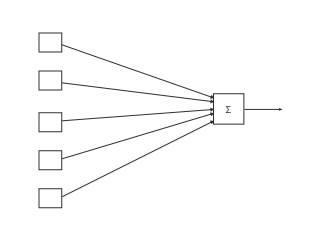
\includegraphics[width=0.50\linewidth]{./figures/perceptron.png}
	\caption{The Perceptron \cite{charniakIntroductionDeepLearning2018}}
	\label{fig:perceptron}
\end{figure}

The main building block of a \ac{MLP} is the \textit{Perceptron}, pictured in figure \ref{fig:perceptron}, a simple computational model initially designed as a binary classificator that mimics biological neurons' behaviour \cite{charniakIntroductionDeepLearning2018}. A neuron might have many inputs $x$ and has a single output $y$. It contains a vector of \textit{weights} $w = (w_1 ... w_m)$, each associated with a single input, and a special weight $b$ called the \textit{bias}. In this context, a perceptron defines a computational operation formulated as equation \ref{eq:perceptron} portrays \cite{charniakIntroductionDeepLearning2018}. \par

\begin{equation} \label{eq:perceptron}
	f(x) =
	\left\{ \begin{aligned} 
		1 &\quad \text{ if } b + \textbf{w} \cdot \textbf{x} > 0\\
		0 &\quad \text{ otherwise} 
	\end{aligned} \right.
\end{equation}

Functions that compute $b + \textbf{w} \cdot \textbf{x} > 0$ are called \textit{linear units} and are identified with $\Sigma$ \cite{charniakIntroductionDeepLearning2018, goodfellowDeepLearning2016}. An activation function $g$ was introduced to enable the output of non-linear data. The default recommendation is the \textit{Rectified Linear Unit} (\textit{ReLU}), with the Logistic curve (sigmoid) also being very common \cite{goodfellowDeepLearning2016}.  \par
Feedforward networks are composed of an input layer formed by the vector of input values, an arbitrary number of hidden layers and an output layer, which is the last layer of neurons \cite{charniakIntroductionDeepLearning2018}. The greater the amount of layers the higher the \textit{depth} of the network \cite{charniakIntroductionDeepLearning2018, goodfellowDeepLearning2016}. \par
On its own, the model amounts only to a complex function. Still, with real-world correspondence between input values and associated outputs, a feedforward network can be trained to approximate the unknown function of the environment. In more concrete terms, this involves updating all of the different weight and bias values of each neuron to achieve an output as close as possible to the real or desired value or minimize the total loss, which indicates how distant the network model is to the real function to approximate \cite{charniakIntroductionDeepLearning2018, goodfellowDeepLearning2016}. \textit{Loss functions} are used to calculate this value.

\begin{figure}
	\centering
	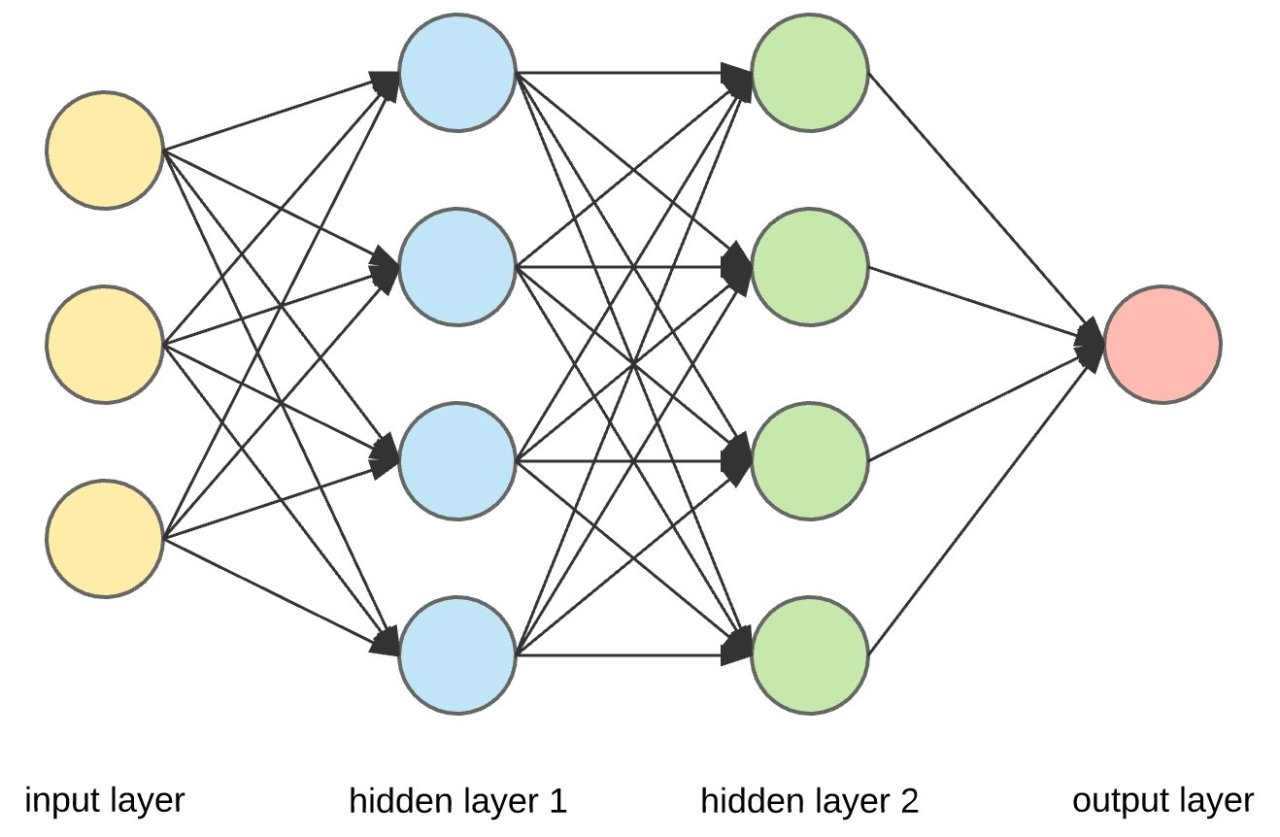
\includegraphics[width=0.50\linewidth]{./figures/fnn.jpg}
	\caption{Architecture of a Feedforward Neural Network \cite{FeedforwardNeuralNetwork}}
	\label{fig:fnn}
\end{figure}


\section{Reinforcement Learning} \label{sec:back-rl}

\begin{comment}
	* SAC
	* DDPG
	* DQN
\end{comment}

\textbf{\ac{RL}} consists of a field and a class of machine learning algorithms that study how to learn to take good sequences of actions to achieve a goal associated with a maximizing received numerical reward \cite{brunskillCS234ReinforcementLearning}. The main objective is to maximize the received cumulative reward by trying between the available actions and discovering which ones yield the most reward \cite{suttonReinforcementLearningIntroduction2014}. This sequential decision-making process becomes more complex when a delayed reward is considered, given that an action with immediate reward may not always reflect the delayed consequences of that decision \cite{suttonReinforcementLearningIntroduction2014}. It's also the learner's job to consider this during the learning process. These concepts of \textit{delayed reward} and \textit{trial-and-error search} make up the most important characteristics of Reinforcement Learning \cite{suttonReinforcementLearningIntroduction2014}. The classic formalisation of this problem is the \ac{MDP} through defining the agent-environment interaction process, explained in the following subsection \ref{sec:back-mpd}. \par 

A major challenge in this machine learning paradigm is the trade-off between \textit{exploring} new unknown actions and \textit{exploiting} the already known "good" actions \cite{suttonReinforcementLearningIntroduction2014}. To choose the sequence of actions that return the highest reward, the agent must choose actions it found effective in similar past situations or *exploit* what it learned from experience. Furthermore, given that the agent may not know the action-reward mappings initially, it has to \textit{explore} possible actions that were not selected previously or may initially seem to yield a low reward to compute accurate reward estimates. The main problem is that neither exploitation nor exploration can be favoured exclusively without failing at the task \cite{suttonReinforcementLearningIntroduction2014}. Additionally, an agent's environment is uncertain, and changes in the environment's dynamics may also involve re-estimating action rewards. \par


In conclusion, \ac{RL} techniques enable the implementation of sequential decision-making agents that seek to maximize a reward signal analogous to an explicit (complex) goal. The agents need to balance between actions that yield a reward on posterior time steps and actions that produce immediate rewards. In addition, these agents are also faced with the task of balancing the exploitation of information from past experiences and the exploration of new decision paths that could potentially return a higher reward down the road \cite{suttonReinforcementLearningIntroduction2014}.  \par



\subsection{Markov Decision Process} \label{sec:back-mpd}
\acfp{MDP} are a classical formalization of a sequential decision-making process, constituting the mathematical definition of the \ac{RL} problem \cite{suttonReinforcementLearningIntroduction2014, moralesGrokkingDeepReinforcement2020}. Beyond estimating potential rewards for the available actions, the problem defined by \acp{MDP} involves learning which actions are optimal in specific situations, i.e. learning a mapping between states of the environment and actions \cite{suttonReinforcementLearningIntroduction2014}. 

The central component of \acp{MDP} is the agent, which acts as a decision-maker and learns from interactions with the environment it's inserted. In a continuous process, the agent takes actions that affect the environment's state, which in turn presents new situations \cite{suttonReinforcementLearningIntroduction2014}. The environment also responds with the reward signals which the agent aims to maximize over time through its decision process.

\begin{figure}
	\centering
	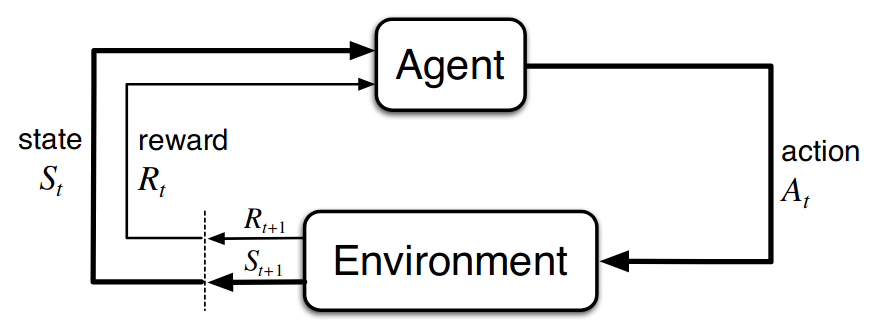
\includegraphics[width=0.75\linewidth]{./figures/mpd.png}
	\caption{Agent-environment interaction in a \acs{MDP}  \cite{suttonReinforcementLearningIntroduction2014}}
	\label{fig:mpd-interaction}
\end{figure}

Formally, the agent-environment interactions, as figure \ref{fig:mpd-interaction} entails, occur in a sequence of discrete time steps $t$, where at each step, the agent receives a representation of the state of the environment $S_t \in \mathcal{S}$ which is used to select an appropriate action $A_t \in \mathcal{A}(s)$, where $\mathcal{S}$ is the set of possible states called the \textit{state space} and $\mathcal{A}(s)$ is the set of available actions for state $s$ \cite{suttonReinforcementLearningIntroduction2014, moralesGrokkingDeepReinforcement2020}. In the next step, the agent receives, as a consequence of its decision, a numerical reward signal $R_{t+1} \in \mathcal{R} \subset \mathbb{R}$ and is faced with a new state $S_{t +1}$ \cite{suttonReinforcementLearningIntroduction2014}. Ultimately, the MDP agent follows a logical sequence that occurs as equation \ref{eq:mpd-sequence} states. The collection of a state $S_t$, action taken $A_{t+1}$, reward $R_{t+1}$ received and next state $S_{t+1}$ constitutes an \textit{experience tuple} \cite{moralesGrokkingDeepReinforcement2020}.

\begin{equation} \label{eq:mpd-sequence}
	S_0, A_0, R_1, S_1, A_2, R_2, S_2, A_2, R_3, \dots
\end{equation}

In addition, when the set of possible actions, states and rewards ($\mathcal{A}$, $\mathcal{S}$ and $\mathcal{R}$) are finite, the \ac{MDP} is said to be \textit{finite} \cite{suttonReinforcementLearningIntroduction2014}. This results in $S_t$ and $R_t$ having well-defined discrete probability distributions in function of the preceding state and chosen action \cite{suttonReinforcementLearningIntroduction2014}. Therefore, the probability of receiving a particular reward and state given the previous state and selected action, which characterizes a finite MPD's dynamics, may be characterized by function $p$ defined in equation \ref{eq:mdp-dynamics}
\begin{equation} \label{eq:mdp-dynamics}
	p(s',r|s,a) \doteq Pr\{S_t = s', R_t = r | S_{t-1} = s, A_{t-1} = a\}
\end{equation}

For all $s, s' \in \mathcal{S}$, $r \in \mathcal{R}$ and $a \in \mathcal{A}(s)$, where $\doteq$ denotes a mathematical formal defintion. This encompasses the assumption that the probability of each possible state, $S_t$, and reward, $R_t$, pair is only dependent on the preceding state, $S_{t-1}$, and action taken, $A_{t-1}$ \cite{suttonReinforcementLearningIntroduction2014}. Instead of observing this as a restriction on the decision process, it's more convenient to view it as a constraint on the state variable, considering that it must contain all the necessary information from experience to make a valuable decision in the immediate step. If this condition is satisfied, the state is declared to have the \textit{markov property} \cite{suttonReinforcementLearningIntroduction2014}. \par
From function $p$ in equation \ref{eq:mdp-dynamics}, the state-transtion probabilities, also called the \textit{transition function}, can be computed as described by equation \ref{eq:mpd-transition} \cite{suttonReinforcementLearningIntroduction2014, moralesGrokkingDeepReinforcement2020}.

\begin{equation} \label{eq:mpd-transition}
	p(s'|s,a) \doteq Pr\{S_t = s'|S_{t-1} = s, A_{t-1} = a\} = \sum_{r \in \mathcal{R}} p(s',r|s,a)
\end{equation}

In addition, the expected rewards can be calculated for state-action pairs (equation \ref{eq:mpd-reward-sa}) or state-action-next-action triples (equation \ref{eq:mpd-reward-sas'}) \cite{suttonReinforcementLearningIntroduction2014, moralesGrokkingDeepReinforcement2020}.

\begin{equation} \label{eq:mpd-reward-sa}
	r(s,a) \doteq \mathbb{E}[R_t | S_{t-1} = s, A_{t-1} = a] = \sum_{r \in \mathcal{R}} r \sum_{s' \in \mathcal{S}} p(s', r|s,a)
\end{equation}
\begin{equation} \label{eq:mpd-reward-sas'}
	r(s,a,s') \doteq \mathbb{E}[R_t | S_{t-1} = s, A_{t-1} = a, S_t = s'] = \sum_{r \in \mathcal{R}} r \frac{p(s',r|s,a)}{p(s'|s,a)}
\end{equation}

\subsection{Rewards and Returns}

As stated in the previous subsections, the main goal of a \ac{RL} agent defined by the numeric reward signal, $R_t \in \mathbb{R}$, it receives from the environment \cite{suttonReinforcementLearningIntroduction2014}. In this context, the agent's objective is to maximize the total reward it receives, considering not only immediate but also the cumulative reward over time. In the ubiquitous work of \cite{suttonReinforcementLearningIntroduction2014}, the \textit{reward hypothesis} is stated as follows:

\begin{displayquote}
	That all of what we mean by goals and purposes can be well thought of as the maximization of the expected value of the cumulative sum of a received scalar signal (called reward). \cite{suttonReinforcementLearningIntroduction2014}
\end{displayquote}
This also entails that the process of reward maximization from the agent has to be closely tied to it achieving its defined goals in a practical sense. Otherwise, the agent will fail at fulfilling the desired objectives \cite{suttonReinforcementLearningIntroduction2014}.

Formally, the goal of an \ac{RL} agent can be defined by the maximization of the cumulative reward received of time called the \textit{expected return}, $\text{Return}_t$ \cite{suttonReinforcementLearningIntroduction2014}.

\begin{equation} \label{eq:expected-return}
	\text{Return}_t \doteq R_{t+1} + R_{t+2} + R_{t+3} + \cdots + R_T
\end{equation}

$T$ describes the final time step. This definition can be applied in domains with a natural notion of a terminal state or final time step. In these cases, the agent-environment interaction process can be broken into logically independent subsequences called \textit{episodes} \cite{suttonReinforcementLearningIntroduction2014}. Each episode ends in a special state, called the terminal state, restarting a new sequence of states and actions completely independent from the previous episode \cite{suttonReinforcementLearningIntroduction2014}. In this context, episodes can be considered to end in the same terminal state, with different accumulated rewards for the different outcomes \cite{suttonReinforcementLearningIntroduction2014}.

In contrast, there are situations where the decision-making process doesn't divide itself into logically identifiable episodes but goes on indefinitely. In this case, $T = \infty$ and according to equation \ref{eq:expected-return}, the expected return the agent aims to maximize would be infinite \cite{suttonReinforcementLearningIntroduction2014}. In this manner, another concept is added in the expected return definition called the \textit{discount rate}, $\gamma$ where $0 \leq \gamma \leq 1$, representing how strongly the agent should account for future rewards in the expected return calculations, as equation \ref{eq:expected-discounted-return} \cite{suttonReinforcementLearningIntroduction2014}.

\begin{equation} \label{eq:expected-discounted-return}
	\text{Return}_t \doteq R_{t+1} + \gamma R_{t+2} + \gamma^2 R_{t+3} + \cdots = \sum^\infty_{k = 0} \gamma^k R_{t+k+1}
\end{equation}

From this equation, we can compute the expected discounted return on a given time step $t$ in the function of the immediate reward signal received and the expected return for the next time step $t +1$, which eases the job of calculating expected returns for reward sequences \cite{suttonReinforcementLearningIntroduction2014}. This is entailed by equation \ref{eq:expected-discounted-next}.
\begin{equation} \label{eq:expected-discounted-next}
	\text{Return}_t = R_{t+1} + \gamma G_{t+1}
\end{equation}

In this manner, a \ac{MDP} can be defined by a tuple with a state space $\mathcal{S}$, an action space $\mathcal{A}$, a transition function $p$, a reward function $r$ and a discount factor $\gamma$, as equation \ref{eq:mdp-tuple} portrays \cite{brunskillCS234ReinforcementLearning}.

\begin{equation} \label{eq:mdp-tuple}
	M = (\mathcal{S}, \mathcal{A}, p, r, \gamma)
\end{equation}

\subsection{Policies and Value Functions}

\ac{RL} techniques typically involve the estimation of what is understood as \textit{value functions}, functions that estimate the expected return based on the current state value or state-action pair. This characterizes how good is for an agent to be in a specific state or to take an action in a specific state, respectively, using the expected return to characterize the overall \textit{goodness} of these scenarios \cite{suttonReinforcementLearningIntroduction2014, moralesGrokkingDeepReinforcement2020}. These functions are tied to a specific way of determining the action in a given state. Formally, this is defined as a \textit{policy} $\pi$, that defines the probability $\pi(a|s)$ of taking action $a$ in state $s$ \cite{suttonReinforcementLearningIntroduction2014}. In this context, the \textit{state-value function}, $v_\pi(s)$ and \textit{action-value functions} $q_\pi(s,a)$ for policy $\pi$ can be defined by equations \ref{eq:state-value-funtion} and \ref{eq:action-value-function}, respectively \cite{suttonReinforcementLearningIntroduction2014}.
\begin{equation} \label{eq:state-value-funtion}
	v_\pi(s) \doteq \mathbb{E}_\pi[\text{Return}_t | S_t = s], \forall s \in \mathcal{S}
\end{equation}
\begin{equation} \label{eq:action-value-function}
	q_\pi(s,a) \doteq \mathbb{E}_\pi[\text{Return}_t | S_t = s, A_t = a]    
\end{equation}

The utility of such functions rely on the possibility of estimating them with regard to past experience of the agent \cite{suttonReinforcementLearningIntroduction2014}. A fundamental property of value functions is that it can, as was the case with the expected return (equation \ref{eq:expected-discounted-next}), satisfy recursive relationships with the next immediate value as equation \ref{eq:bellman-equation-v} entails \cite{suttonReinforcementLearningIntroduction2014}. This equation is called the \textit{Bellman equation for $v_\pi$}, which characterizes the relationship between the value of current and subsequent states.

\begin{equation} \label{eq:bellman-equation-v}
	v_\pi \doteq \sum_{a \in \mathcal{A}(s)} \pi(a|s) \sum_{s' \in \mathcal{S}, r \in \mathcal{R}} p(s',r|s,a) [r + \gamma v_\pi (s')]
\end{equation}
\begin{equation} \label{eq:action-value-function}
	q_\pi(s,a) \doteq \sum\mathbb{E}_\pi[\text{Return}_t | S_t = s, A_t = a]    
\end{equation}


\subsection{Types of \ac{RL}}


\begin{figure}
	\centering
	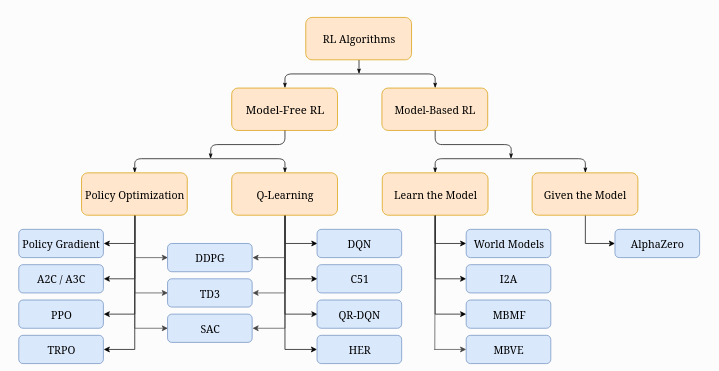
\includegraphics[width=0.75\linewidth]{./figures/rl_algorithms.png}
	\caption{Taxonomy of algorithms in modern \ac{RL} \cite{openaiSpinningDocumentation}}
	\label{fig:rl-algorithms}
\end{figure}

Regarding \ac{RL} algorithms, they can be divided into model-free and model-based techniques \cite{openaiSpinningDocumentation}. These categories are distinguished by whether an agent uses a provided or learned \textit{model} of the set of transition and reward functions, another optional element of \ac{RL} techniques \cite{moralesGrokkingDeepReinforcement2020, openaiSpinningDocumentation}. In the positive case, the method is said to be model-based, otherwise, it's model-free. Having an accurate model of the environment allows the \ac{RL} agent to focus on planning ahead by calculating future scenarios and creating policies based on the results of the planning process. An example of a famous system of this kind is AlphaZero \cite{silverMasteringChessShogi2017}. However, in most cases, agents can't access a ground-truth model of the environment, leaving only the scenario where an agent learns a model purely from experience. This creates several challenges, the most prominent of which relies on the fact that the model, in most times, doesn't fully capture the environment's transition dynamics, equipping it with bias in relation to the actual dynamics. With this, learning how to generalise the model to real-world environments so that the bias is not over-exploited becomes a very complex task \cite{openaiSpinningDocumentation}.  Model-free algorithms can be also further divided into Q-learning and Policy Aproximmation techniques. \par
Furthermore, algorithms can also be subdivided into on-policy and off-policy methods. \cite{moralesGrokkingDeepReinforcement2020} On-policy algorithms evaluate and improve a single policy used to determine the agent's behaviour \cite{moralesGrokkingDeepReinforcement2020}. The methods under the policy optimization category such as A2C and A3C \cite{mnihAsynchronousMethodsDeep2016} or the \ac{PPO} \cite{schulmanProximalPolicyOptimization2017} almost always fall into this label. In contrast, off-policy algorithms learn how to improve a different target policy based on the results that arise from the policy used to determine the system behaviour initially \cite{moralesGrokkingDeepReinforcement2020}. Such approaches include Q-Learning algorithms such as \acp{DQN} \cite{mnihHumanlevelControlDeep2015, openaiSpinningDocumentation}. \ac{DDPG} \cite{lillicrapContinuousControlDeep2019} combines policy optimization with q-learning, consisting of an off-policy method that learns both a q-function and a policy. \ac{DDPG} constitutes the adaption of q-learning methods to continuous action spaces \cite{openaiSpinningDocumentation}. Another example of an off-policy algorithm is the \ac{SAC} \cite{haarnojaSoftActorCriticOffPolicy2018} method, which bridges stochastic policy optimization with the \ac{DDPG} approach and has entropy regularization as one of its central features, which translates into training a policy that maximizes the expected return and entropy, a measure of randomness in the policy \cite{openaiSpinningDocumentation}. \par
Lastly, with the advent of deep learning becoming one of the most ubiquitous techniques in machine learning, \ac{RL} algorithms have evolved beyond the traditional tabular methods \cite{moralesGrokkingDeepReinforcement2020}. Traditional \ac{RL} has evolved to \ac{DRL}, which studies how to use deep neural networks in \ac{RL} problems to leverage their generalization abilities for solving more complex problems.

\section{Graph Representation Learning} \label{sec:back-grl}

Several objects and problems can be naturally expressed in the real world using graphs, such as social networks, power grids, transportation networks, recommendation systems or drug discovery. The usefulness of such representations is tied to how they instinctively represent the complex relationships between objects. However, graph data is often very sparse and complex, and their sophisticated structure is difficult to deal with \cite{liuIntroductionGraphNeural2020, zhaoRepresentationLearning2022}. \par

Furthermore, the performance of machine learning models strongly relies not only on their design but also on good representations of the underlying information \cite{liuIntroductionGraphNeural2020}.  Ineffective representations, on the one hand, can lack important graph features and, on the other, can carry vast amounts of redundant information, affecting the algorithms' performance in leveraging the data for different analytical tasks \cite{liuIntroductionGraphNeural2020, wuGraphNeuralNetworks2022}. \par

In this context, \textbf{Graph Representation Learning} studies how to learn the underlying features of graphs to extract a minimal but sufficient representation of the graph attributes and structure \cite{hamiltonGraphRepresentationLearning, zhaoRepresentationLearning2022, cuiGraphRepresentationLearning2022}. Currently, the improvements in deep learning allow representation learning techniques consisting of the composition of multiple non-linear transformations that yield more abstract and, ultimately, more useful representations of graph data \cite{cuiGraphRepresentationLearning2022}. 

\section{Graph Neural Networks} \label{sec:back-gnn}
 
\begin{comment}
	* GraphSAGE
	\cite{scarselliGraphNeuralNetwork2009}
\end{comment}

In the present, deep learning and \ac{ANN} have become one of the most prominent approaches in Artificial Intelligence research \cite{cuiGraphRepresentationLearning2022}. Approaches such as recurrent neural networks and convolutional networks have achieved remarkable results on Euclidean data, such as images or sequence data, such as text and signals \cite{wuGraphNeuralNetworks2022a}. Furthermore, techniques regarding deep learning applied to graphs have also experienced rising popularity among the research community, more specifically \textbf{\acp{GNN}} that became the most successful learning models for graph-related tasks across many application domains \cite{cuiGraphRepresentationLearning2022, wuGraphNeuralNetworks2022a}. \par

The main objective of \acp{GNN} is to update node representations with representations from their neighbourhood iteratively \cite{tangGraphNeuralNetworks2022}. Starting at the first representation $H^0 = X$, each layer encompasses two important functions:
\begin{itemize}
	\item \textbf{Aggregate}, in each node, the information from their neighbours
	\item \textbf{Combine} the aggregated information with the current node representations
\end{itemize}

The general framework of \acp{GNN}, outlined in \cite{tangGraphNeuralNetworks2022}, can be defined mathematically as follows: \\ \\
Initialization: $H^0 = X$ \\
For $k = 1, 2, \dots, K$
\begin{gather*}
	a^k_v = \text{AGGREGATE}^k\{H^{k-1}_u : u \in N(v)\} \\
	H^k_v = \text{COMBINE}^k\{H^{k-1}_u, a^k_v\}       
\end{gather*}

Where $N(v)$ is the set of neighbours for the $v$-th node. The node representations $H^K$ in the last layer can be treated as the final representations, which sequentially can be used for other downstream tasks \cite{tangGraphNeuralNetworks2022}.


\subsection{Graph Convolutional Network}

A \textbf{\ac{GCN}} \cite{kipfSemiSupervisedClassificationGraph2017} is a popular architecture of \acp{GNN} praised by its simplicity and effectiveness in a variety of tasks \cite{liuIntroductionGraphNeural2020, tangGraphNeuralNetworks2022}. In this model, the node representations in each layer are updated according to the following convolutional operation:

\begin{equation} \label{eq:graph-convolution}
	H^{k+1} = \sigma(\tilde{D}^{-\frac{1}{2}} \tilde{A} \tilde{D}^{-\frac{1}{2}} H^k W^k)  
\end{equation}

$Ã = A + I$ - Adjacency Matrix with self-connections \\
$I \in \mathbb{R}^{N \times N}$ - Identity Matrix \\
$\tilde{D}$ - Diagonal Matrix,  with $\tilde{D}_{ii} = \sum_j Ã_{ij}$ \\
$\sigma$ - Activation Function \\
$W^k \in \mathbb{R}^{F \times F'}$ - Laywise linear transformation matrix ($F$ and $F'$ are the dimensions of node representations in the $k$-th and $(k + 1)$ layer, respectively) \\

$W^k \in \mathbb{R}^{F \times F'}$ is a layerwise linear transformation matrix that is trained during optimization \cite{tangGraphNeuralNetworks2022}. The previous equation \ref{eq:graph-convolution} can be dissected further to understand the \textit{AGGREGATE} and \textit{COMBINE} function definitions in a \ac{GCN} \cite{tangGraphNeuralNetworks2022}. For a node $i$, the representation updating equation can be reformulated as:

\begin{gather}
	H^k_i = \sigma(\sum_{j \in \{N(i) \cup i\}} \frac{\tilde{A}_{ij}}{\sqrt{\tilde{D}_{ii} \tilde{D}_{jj}}} H^{k-1}_j W^k) \\
	H^k_i = \sigma(\sum_{j \in N(i)} \frac{A_{ij}}{\sqrt{\tilde{D}_{ii} \tilde{D}_{jj}}} H^{k-1}_j W^k) + \frac{1}{\tilde{D}_i} H^{k-1} W^k)
\end{gather}

In the second equation, the \textit{AGGREGATE} function can be observed as the weighted average of the neighbour node representations \cite{tangGraphNeuralNetworks2022}. The weight of neighbour $j$ is defined by the weight of the edge $(i,j)$, more concretely, $A_{ij}$ normalized by the degrees of the two nodes \cite{tangGraphNeuralNetworks2022}. The \textit{COMBINE} function consists of the summation of the aggregated information and the node representation itself, where the representation is normalized by its own degree \cite{tangGraphNeuralNetworks2022}.

\subsection*{Spectral Graph Convolutions}

Regarding the connection between GCNs an spectral filters defined on graphs, spectral convolutions can be defined as the multiplication of a node-wise signal $x \in \mathbb{R}^N$ with a convolutional filter $g_\theta = diag(\theta)$ in the \textit{Fourier domain} \cite{liuIntroductionGraphNeural2020, tangGraphNeuralNetworks2022}, formally:

\begin{equation}    
	g_\theta \star \text{x} = U_{g_\theta} U^T \text{x}
\end{equation}

$\theta \in \mathbb{R}^N$ - Filter parameter \\
$U$ - Matrix of eigenvectors of the normalized graph Laplacian Matrix $L = I_N - D^{-\frac{1}{2}} AD^{-\frac{1}{2}}$ \\

The eigendecomposition of the Laplacian matrix can also be defined by $L = U \Lambda U^T$ with $\Lambda$ serving as the diagonal matrix of eigenvalues and $U^T \text{x}$ is the graph Fourier transform of the input signal $\text{x}$ \cite{tangGraphNeuralNetworks2022}. In a practical context, $g_\theta$ is the function of eigenvalues of the normalized graph Laplacian matrix $L$, that is $g^\theta(\Lambda)$ \cite{liuIntroductionGraphNeural2020, tangGraphNeuralNetworks2022}. Computing this is a problem of quadratic complexity to the number of nodes $N$, something that can be circumvented by approximating $g_\theta (\Lambda)$ with a truncated expansion of Chebyshev polynomials $T_k(x)$ up to $K$-th order \cite{liuIntroductionGraphNeural2020, tangGraphNeuralNetworks2022}:

\begin{equation}
	g_{\theta'}(\Lambda) = \sum^K_{k=0} \theta'_k T_k(\tilde{\Lambda})    
\end{equation}

$\tilde{\Lambda} = \frac{2}{\lambda_\text{max}} \Lambda - \text{I}$  \\
$\lambda_\text{max}$ - Largest eigenvalue of $L$ \\
$\theta' \in \mathbb{R}^N$ - Vector of Chebyshev coefficients \\
$T_k(x)$ - Chebyshev polynomials \\
$T_k(x) = 2 x T_{k - 1} (x) - T_{k - 2}(x)$ with $T_0(x) = 1$ and $T_1(x) = x$ \\

By combining this with the previous equation, the first can be reformulated as:

\begin{equation}
	g_\theta \star \text{x} = \sum^K_{k=0} \theta'_k T_k(\tilde{L}) \text{x}
\end{equation}

$\tilde{L} = \frac{2}{\lambda_\text{max}} L - I$ 

From this equation, it can be observed that each node depends only on the information inside the $K$-th order neighbourhood and with this reformulation, the computation of the equation is reduced to $O(|\xi|)$, linear to the number of edges $\xi$ in the original graph $G$. \par

To build a neural network with graph convolutions, it's sufficient to stack multiple layers defined according to the previous equation, each followed by a nonlinear transformation. However, the authors of \ac{GCN} \cite{kipfSemiSupervisedClassificationGraph2017} proposed limiting the convolution number to $K = 1$ at each layer instead of limiting it to the explicit parametrization by the Chebyshev polynomials. This way, each level only defines a linear function over the Laplacian Matrix $L$, maintaining the possibility of handling complex convolution filter functions on graphs by stacking multiple layers \cite{kipfSemiSupervisedClassificationGraph2017, tangGraphNeuralNetworks2022}. This means the model can alleviate the overfitting of local neighbourhood structures for graphs whose node degree distribution has a high variance \cite{kipfSemiSupervisedClassificationGraph2017, tangGraphNeuralNetworks2022}.

At each layer, it can further considered $\lambda_\text{max} \approx 2$, which the neural network parameters could accommodate during training \cite{tangGraphNeuralNetworks2022}. With these simplifications, the equation is transformed into:
\begin{equation}
	g_{\theta'} \star \text{x} \approx \theta'_0 \text{x} + \theta'_1 \text{x} (L - I_N) \text{x} = \theta'_0 \text{x} - \theta'_1 D^{-\frac{1}{2}} AD^{-\frac{1}{2}}
\end{equation}

$\theta'_0$ and $\theta'_1$ - Free parameters that can be shared over the entire graph \\


The number of parameters can, in practice, be further reduced, minimising overfitting and minimising the number of operations per layer as well \cite{tangGraphNeuralNetworks2022} as equation \ref{eq:gcn-reduced-param} entails.

\begin{equation} \label{eq:gcn-reduced-param}
	g_\theta \star \text{x} \approx \theta (I + D^{-\frac{1}{2}} AD^{-\frac{1}{2}}) \text{x}
\end{equation}

$\theta = \theta'_0 = - \theta'_1$

One potential problem is the $I_N + D^{-\frac{1}{2}} AD^{-\frac{1}{2}}$ matrix whose eigenvalues fall in the $[0,2]$ interval. In a deep GCN, the repeated utilization of the above function often leads to an exploding or vanishing gradient, translating into numerical instabilities \cite{liuIntroductionGraphNeural2020, tangGraphNeuralNetworks2022}. In this context, the matrix can be further renormalized by converting $I + D^{-\frac{1}{2}} AD^{-\frac{1}{2}}$ into $\tilde{D}^{-\frac{1}{2}} \tilde{A}\tilde{D}^{-\frac{1}{2}}$ \cite{liuIntroductionGraphNeural2020, tangGraphNeuralNetworks2022}. 
In this case, only the scenario where there is one feature channel and one filter is considered which can be then generalized to an input signal with $C$ channels $X \in \mathbb{R}^{N \times C}$ and $F$ filters (or hidden units) \cite{liuIntroductionGraphNeural2020, tangGraphNeuralNetworks2022}:
\begin{equation}
	H = \tilde{D}^{-\frac{1}{2}} \tilde{A}\tilde{D}^{-\frac{1}{2}}XW    
\end{equation}

$W \in \mathbb{R}^{C \times F}$ - Matrix of filter parameters \\
$H$ - Convolved Signal Matrix \\


\subsection{Graph Attention Network}

\textbf{\ac{GAT}} \cite{velickovicGraphAttentionNetworks2018} is another type of \acp{GNN} that focuses on leveraging an attention mechanism to learn the importance of a node's neighbours. In contrast, the \ac{GCN} uses edge weight as importance, which may not always represent the true strength between two nodes \cite{tangGraphNeuralNetworks2022, velickovicGraphAttentionNetworks2018}.

The Graph Attention Layer defines the process of transferring the hidden node representations at layer $k - 1$ to the next node presentations at $k$. To ensure that sufficient expressive power is attained to allow the transformation of the lower-level node representations to higher-level ones, a linear transformation $W \in \mathbb{R}^{F \times F'}$ is applied to every node, followed by the self-attention mechanism, which measures the attention coefficients for any pair of nodes through a shared attentional mechanism $a: \mathbb{R}^{F'} \times \mathbb{R}^{F'} \rightarrow \mathbb{R}$ \cite{tangGraphNeuralNetworks2022, velickovicGraphAttentionNetworks2018}. In this context, relationship strength $e_{ij}$ between two nodes $i$ and $j$ can be calculated by:
\begin{equation}
	e_{ij} = a(W H^{k - 1}_i, W H^{k - 1}_j)
\end{equation}

$H^{k - 1}_i \in \mathbb{R}^{N \times F'}$ - Column-wise vector representation of node $i$ at layer $k - 1$ ($N$ is the number of nodes and $F$ the number of features per node) \\
$W \in \mathbb{R}^{F \times F'}$ - Shared linear transformation \\
$a: \mathbb{R}^{F'} \times \mathbb{R}^{F'} \rightarrow \mathbb{R}$ - Attentional Mechanism \\
$e_{ij}$ - Relationship Strength between nodes $i$ and $j$ \\

Theoretically, each node can attend to every other node on the graph, although it would ignore the graph's topological information in the process. A more reasonable solution is to only attend nodes in the neighbourhood \cite{velickovicGraphAttentionNetworks2018, tangGraphNeuralNetworks2022}. In practice, only first-order node neighbours are used, including the node itself, and to make the attention coefficients comparable across the various nodes, they are normalized with a \textit{softmax} function:
$$ \alpha_{ij} = \text{softmax}_j(\{e_{ij}\}) = \frac{exp(e_{ij})}{\sum_{l \in N(i)} exp(e_{il})}$$

Fundamentally, $\alpha_{ij}$ defines a multinomial distribution over the neighbours of node $i$, which can also be interpreted as a transition probability from node $i$ to each node in its neighbourhood \cite{tangGraphNeuralNetworks2022}. 
In the original work \cite{velickovicGraphAttentionNetworks2018}, the attention mechanism is defined as a single-layer Feedforward Neural Network that includes a linear transformation with weigh vector $W_2 \in \mathbb{R}^{1 \times 2 F'}$ and a LeakyReLU nonlinear activation function with a negative input slope $\alpha = 0.2$ \cite{tangGraphNeuralNetworks2022, velickovicGraphAttentionNetworks2018}. More formally, the attention coefficients are calculated as follows:
\begin{equation}
	\alpha_{ij} = \frac{ \text{exp}( \text{LeakyReLU}( W_2 [W H^{k - 1}_i || W H^{k - 1}_j]))}{ \sum_{l \in N(i)} \text{exp}( \text{LeakyReLU}( W_2 [W H^{k - 1}_i || W H^{k - 1}_l])) }
\end{equation}

$||$ - Vector concatenation operation

The novel node representation is a linear composition of the neighbouring representations with weights determined by the attention coefficients \cite{velickovicGraphAttentionNetworks2018, tangGraphNeuralNetworks2022}, formally:
\begin{equation}
	H^k_i = \sigma(\sum_{j \in N(i)} \alpha_{ij} W H^{k - 1}_j) 
\end{equation}


\subsection*{Multi-head Attention}

Multi-head attention can be used instead of self-attention, determining a different similarity function over the nodes. An independent node representation can be obtained for each attention head according to the equation bellow \cite{velickovicGraphAttentionNetworks2018, tangGraphNeuralNetworks2022}. The final representation is a concatenation of the node representations learned by different heads, formally:
$$ H^k_i = \Big\Vert^T_{t=1} \sigma(\sum_{j \in N(i)} \alpha^t_{ij} W^t H^{k-1}_j)$$

$T$ - Number of attention heads \\
$\alpha^t_{ij}$ - attention coefficient computed from the $t$-th attention head \\
$W^t$ - Linear transformation matrix of the $t$-th attention head \\

Lastly, the author also mentions that other pooling techniques can be used in the final layer for combining the node representations from different heads, for example, the average node representations from different attention heads \cite{velickovicGraphAttentionNetworks2018, tangGraphNeuralNetworks2022}.
\begin{equation}
	H^k_i = \sigma(\frac{1}{T} \sum^T_{t = 1} \sum_{j \in N(i)} \alpha^t_{ij} W^t H^{k-1}_j)
\end{equation}


\section{Smart Grid Services} \label{sec:back-smart-grid}

Given the global ecological emergency and the increasing energetic crisis, there is a necessity for advancements in energy distribution and transmission systems now more than ever. To fulfil the need for energy sustainability, traditional centralized distribution grids must be adapted to, on the one hand, accommodate the rise of distributed renewable energy sources in corporate and domestic consumers and, on the other, to make more efficient and reliable distribution of energy resources \cite{farhangiPathSmartGrid2010, vijayapriyaSmartGridOverview2011}. \par


\begin{figure}[h!]
	\centering
	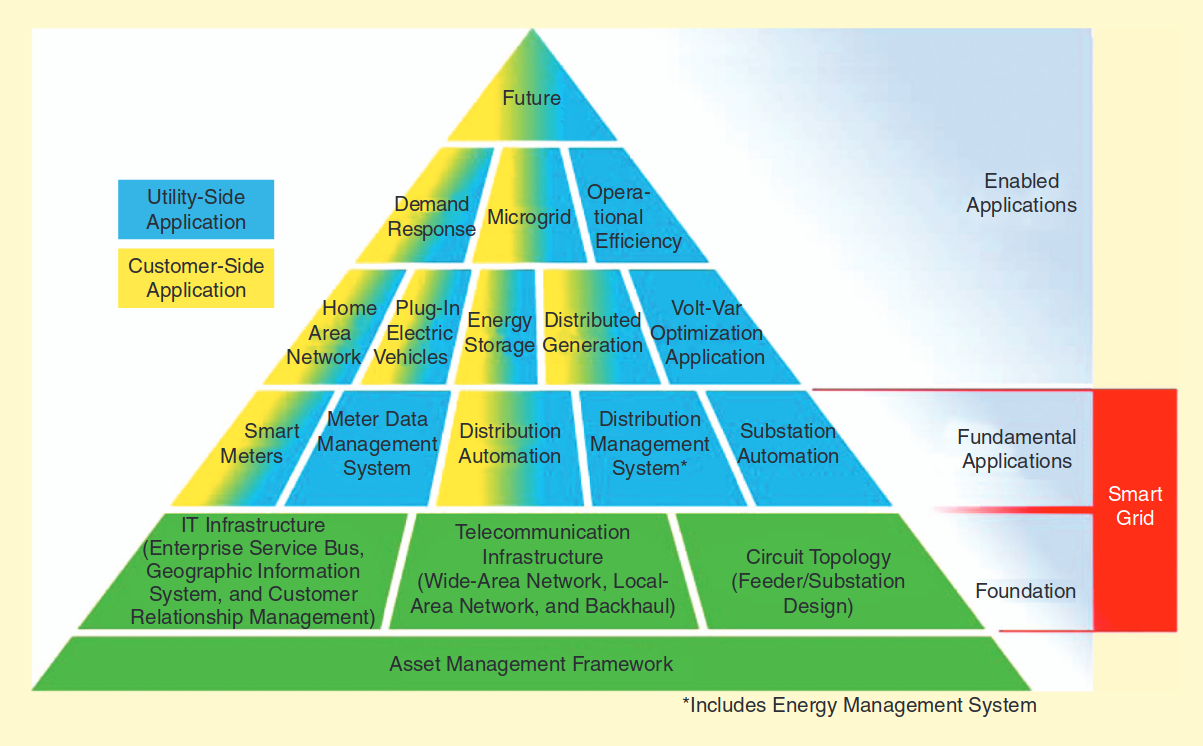
\includegraphics[width=0.74\linewidth]{./figures/smart_grid.png}
	\caption{Smart Grid Capabilities Pyramid \cite{farhangiPathSmartGrid2010}}
	\label{fig:smart-grid}
\end{figure}


The \textit{Smart Grid} or the \textit{Smart Power Grid} conceptualizes this modernization of the electricity network by leveraging the technological advancements in information technology and communication science to create intelligent systems that manage and monitor the distributed generation of energy \cite{bayindirSmartGridTechnologies2016, farhangiPathSmartGrid2010}. Figure \ref{fig:smart-grid} describes the smart grid pyramid, which has asset management at its base. On this foundation, the foundation of the smart grid is laid out by the circuit topology, \acs{IT} systems and telecommunications infrastructure, the basic ingredients for the emergence of fundamental applications such as smart meters and distribution automation \cite{farhangiPathSmartGrid2010}. In turn, these serve as building blocks for creating more intelligent systems that leverage upper-layer applications, enabling the true smart grid capabilities \cite{farhangiPathSmartGrid2010}.

\chapter{Literature Review} \label{chap:literature-review}

\ac{GRL} or Reinforcement Learning on Graphs is a relatively new area in the broader field of machine learning. \ac{GRL} techniques have shown significant progress in solving problems with underlying graph-based representations such as power grid management \cite{liNovelGraphReinforcement2022, chenGraphRepresentationLearningbased2023}, smart transport \cite{xingBilevelGraphReinforcement2023, almasanDeepReinforcementLearning2022} or task offloading \cite{gaoFastAdaptiveTask2023, liGraphReinforcementLearningbased2022}. In this work, the main focus lies on studying the development of \ac{GRL} techniques and subsequent application to smart grid services such as dynamic economic energy dispatch systems \cite{chenScalableGraphReinforcement2023, xingRealtimeOptimalScheduling2023}, residential electricity behavior identification and energy management \cite{chenGraphRepresentationLearningbased2023}, or Volt-VAR regulation \cite{huMultiagentGraphReinforcement2024}.  \par
Research on this topic has significantly increased in the last few years with the improvements of \ac{DRL} techniques and the developments in \acp{GNN} in the mid-2010s \cite{kipfSemiSupervisedClassificationGraph2017, velickovicGraphAttentionNetworks2018, liGatedGraphSequence2016, gaoGraphUNets2019}. \acp{GNN} became the state-of-the-art for solving numerous data mining tasks involving graph-structured data, excelling at classification, link prediction and representation learning \cite{xuHowPowerfulAre2019, nieReinforcementLearningGraphs2023}. This advancement brought more sophisticated \ac{RL} applications on graphs and the surge of a new field studying how to combine the improvements of graph mining and reinforcement learning techniques. \par
In this context, this literature review is divided into the two main approaches in \ac{GRL}, which compromise the popular \ac{GCN} architecture that has been widely researched or leveraging the rising and promising \ac{GAT} architecture. Lastly, other relevant approaches that use different architectures are also listed.


\subsection{Plain GCN-Based GRL Techniques}

A common approach in Graph Reinforcement Learning model implementation is the use of graph convolutions with the \acp{GCN} architecture for leveraging graph-based structures to extract and aggregate the essential features of data in hand and improve the performance of \ac{RL} agents in those environments. The techniques listed in this subsection constitute approaches that integrate a \ac{GCN} with \ac{RL} algorithms.\par
\cite{liNovelGraphReinforcement2022} implements a \ac{GRL} system to improve the decision quality of economic dispatch under high penetration of distributed energy generations. To accomplish this, a \ac{SAC} system is employed with the main objective of finding the optimal action policy for minimizing generation cost with the appropriate reliability concerns. This problem is represented by an undirected graph with nodes describing the power grid elements with their respective attributes and edges describing the underlying energy connections between those units. To extract the structural features of the graph, this work implements a full connected layer to perform feature transformation with a two-layer \ac{GCN} followed by three full connected layers for the non-linear mapping of state-to-action policy in both actor and critic modules. \cite{chenScalableGraphReinforcement2023} develops a similar approach, with both concluding that it significantly reduces learning time for achieving better training results in comparison to plain \ac{SAC} and showing significant improvement on economy and flexibility of the system on more complex and sparse state graphs. The use of \acp{GCN} enables the system to adapt to changes in the state space by leveraging the network's generalization ability.\par
In \cite{xingGraphReinforcementLearningBased2023} a three-layer \ac{GCN} is used to extract node feature and graph topology information and is integrated into a Rainbow-based \cite{hesselRainbowCombiningImprovements2018} \ac{DRL} algorithm for electric vehicle charging guidance. In this article, the testing results show promising performance in reducing operation costs for electric vehicle users, portraying a model with good generalization ability in untrained scenarios. \par
Another interesting implementation of this approach is \cite{chenAutonomousExplorationUncertainty2020}, which studies and compares different solutions for optimizing autonomous exploration under uncertain environments. It analyzes combinations of a single agent Deep Q-Network (DQN) and Advantageous Actor-Critic (A2C) with Graph Convolutional Networks, Gated Graph Recurrent Networks and Graph U-Nets. The paper reports that the GCN-DQN was the model that achieved the highest reward during policy training, followed by the GGNN-A2C model, although in the end, it concludes that the second showed improved scalability in relation to the first model. In \cite{chenGraphRepresentationLearningbased2023} a DQN with a GCN is also used for residential electricity behaviour identification and energy management.

\begin{table}[h!]
	\centering
	\caption{GCN-Based GRL Techniques}
	\begin{tabular}{|P{2cm}|P{2cm}|p{5cm}|  }
		\hline
		\textbf{Reference} & \textbf{DRL Algorithm} & \textbf{Application Domain} \\
		\hline
		\cite{liNovelGraphReinforcement2022}, \cite{chenScalableGraphReinforcement2023} & GCN-SAC & Dynamic economic energy dispatch \\ \hline
		\cite{lengGraphConvolutionalNetworkbased2021} & GCN-SAC & Multi-access Edge Computing \\ \hline
		\cite{yanAutomaticVirtualNetwork2020} & GCN-A3C & Automatic Virtual Network Embeddings \\ \hline
		\cite{wangGCNRLCircuitDesigner2020} & GCN-DDPG & Automatic transistor sizing \\ \hline
		\cite{chenAutonomousExplorationUncertainty2020} & GCN-DQN  & Autonomous Exploration under uncertainty \\  \hline
		\cite{chenGraphRepresentationLearningbased2023} & GCN-DQN & Residential electricity behavior identification and energy management \\ \hline
		\cite{xingGraphReinforcementLearningBased2023} & GCN - Modified Rainbow & Electrical Vehicle Charging Guidance \\ \hline
		\cite{yuanXGNNModelLevelExplanations2020} & GCN-MDP & Interpret GNNs at model-level \\ \hline
		\cite{tangDependentTaskOffloading2020} & GCN-DQ & Task Offloading in Edge Computing \\ \hline
	\end{tabular}
\end{table}




\subsection{Attention-based GRL Techniques}
Another effective approach in extracting relevant topology and graph features relies on using attention mechanisms to weigh different nodes' contributions dynamically. While this encompasses techniques that use the \ac{GAT} architecture, which is a \ac{GNN} design with the attention mechanism at its core, various scholars propose \ac{GCN} approaches integrated with attention mechanisms such as \cite{zhaoLearningSequentialDistribution2022} and \cite{fanAttentionBasedMultiAgentGraph2023}.
\cite{xingRealtimeOptimalScheduling2023} proposes a \ac{DDPG}-based algorithm improved with a \ac{GAT} block with three graph Attention Layers for extracting and learning the topology information for achieve real-time optimal scheduling for \acp{ADN}. This paper compares the obtained test results against a \ac{GCN}-\ac{DDPG} model and shows increased performance over the \ac{GCN} method in reducing cost and power loss. Beyond this, the work demonstrates that the \ac{GAT}'s attention mechanism enables the algorithm to focus on more important nodes and improve the signal-to-noise ratio compared to its \ac{GCN} counterpart. \cite{chenPhysicalassistedMultiagentGraph2023} and propose a multi-agent approach to the same domain but more focused on voltage regulation with a multi-agent \ac{SAC} instead of a single-agent \ac{DDPG} algorithm. \par
In \cite{xingBilevelGraphReinforcement2023}, another model for the electric vehicle charging guidance is proposed, consisting of a bi-level approach of a Rainbow-based algorithm with a \ac{GAT} block. The upper level focuses on the decision-making process regarding charging, while the lower level handles routing. The proposed model proved to be more effective than a shortest distance path-based \cite{xingModellingDrivingCharging2021} and a \ac{DRL}-based \cite{qianDeepReinforcementLearning2020} approach. It suggests that in a future direction, developing \acp{GNN} directly embedded into the \ac{RL} framework might further improve the model's robustness and scalability. \cite{xuRealtimeFastCharging2022} develops a similar approach with a Double-prioritized DQN for the same application domain.
In \cite{zhaoLearningSequentialDistribution2022} and \cite{fanAttentionBasedMultiAgentGraph2023}, the sequential distribution system restoration problem is addressed with a multi-agent \ac{RL} algorithm equipped with a \ac{GCN} with an attention mechanism. In the first case, multi-head attention is used as the convolution kernel for the \ac{GCN} with a \ac{DQN} algorithm. In the second, self-attention is used for improving the centralized training of the used multi-agent actor-critic algorithm, more concretely, by embedding it in the critic networks. At the same time, the \ac{GCN} is integrated into the actor networks for extracting the graph features. Both solutions proved more efficient than traditional \ac{RL} techniques, with the first highlighting its solution generalizability and the second showing increased scalability facing the non-GRL techniques.


\begin{table}[h!]
	\centering
	\caption{Attention-Based GRL Techniques}
	\begin{tabular}{|P{2cm}|P{4cm}|p{6cm}|  }
		\hline
		\textbf{Reference} & \textbf{DRL Algorithm} & \textbf{Application Domain} \\
		\hline
		\cite{xingRealtimeOptimalScheduling2023} & GAT-DDPG & Optimal Scheduling for ADNs  \\ \hline
		\cite{chenPhysicalassistedMultiagentGraph2023}  &  GAT-MASAC  & Multi-agent Voltage Regulation \\ \hline 
		\cite{xingBilevelGraphReinforcement2023} & GAT-Modified Rainbow & Electric Vehicle Charging Guidance \\ \hline
		\cite{xuRealtimeFastCharging2022} & GAT-DQN & Electric Vehicle Charging Guidance \\ \hline 
		\cite{zhaoLearningSequentialDistribution2022} & GCN-DQN & Multi-agent Sequential Distribution System Restoration \\ \hline
		\cite{fanAttentionBasedMultiAgentGraph2023} & GCN-MAAC & Multi-agent Service Restoration \\ \hline
	\end{tabular}
\end{table}


\subsection{Other Approaches}

This subsection includes \ac{GRL} approaches that combine of other \acp{GNN} architectures with \ac{RL} algorithms. In \cite{peiEmergencyControlStrategy2023}, a GraphSAGE network is used with a Deep Dueling Double Q-Network (D3QN) for emergency control of Undervoltage load shedding for power systems with various topologies. The author presents promising results for the GraphSAGE-D3QN model compared to a GCN-D3QN, achieving higher cumulative reward and faster voltage recovery speed, although it required longer decision times. The proposed model performed excellently in the application domain and successfully generalised the learned knowledge to new topology variation scenarios. \par
\cite{zhangLearningDispatchJob2020} focused on solving the Job shop scheduling problem through a priority dispatching rule with a Graph Isomorphism Network \cite{xuHowPowerfulAre2019} and an actor-critic \ac{PPO} algorithm where the GIN is shared between actor and critic networks. The method showed superior performance against other traditional manually designed priority dispatching rule baselines, outperforming them by a large margin.

\begin{comment}
	GCN
	
	\cite{yanGraphCooperationDeep2023} & GCN-DQN & GRU, Multi-agent and Multi-head Attention & Ecological Traffic Signal Control \\ \hline
	
	\cite{luoMultiAgentCollaborativeExploration2019} & GCN-DQN & & Autonomous Exploration under uncertainty \\ \hline
	
	Attention
	\cite{huMultiagentGraphReinforcement2024} & HRGN-MASAC & Multi-agent Vol-VAR Regulation \\ \hline
	
\end{comment}

\section{Conclusion}

In conclusion, \ac{GRL} is very promising field, where several different applications and techniques were already studied. \acp{GNN} architectures such as \ac{GCN} have been extensively applied with DRL algorithms for enabling feature extracting from graph-based state representations \cite{chenScalableGraphReinforcement2023, chenAutonomousExplorationUncertainty2020}. Architectures such as the GraphSAGE and other attention-based have also been successfully applied with very promising results \cite{peiEmergencyControlStrategy2023, xingRealtimeOptimalScheduling2023} in comparison with \acp{GCN}. However, less research regarding their integration with DRL algorithms was discovered. This suggests that a possible improvement and research direction in the development of \ac{GRL} techniques might be connected with exploring the use of different \acp{GNN} architectures and using the rising attention-based techniques.


% !TeX spellcheck = en_GB
\chapter{Methodological Approach} \label{chap:method-approach}

In this chapter, we will formally state the problem this work aims to address, as well as its the proposed solution. In section \ref{sec:problem} the problem statement is exposed, section \ref{sec:requirements} lists the solutions main functional, non-functional and structural requirements, section \ref{sec:arch} addresses the architecture of the solution, section \ref{sec:method} exposes the established methodology and section \ref{sec:work-plan} contains the proposed work plan.

\section{Problem Statement} \label{sec:problem}

\begin{displayquote}
	 \textit{The reviewed literature addressing solutions to sequential decision-making problems in graph-based environments is sparse and scarce, leading to a research gap for comparative and systematic \ac{GRL} approaches analysing scalability under different sized scenarios and adaptability to topology variation.}
\end{displayquote}

As addressed in the previous chapter, graphs are ubiquitous representations that can serve to instinctively represent several problems and their objects. In some network-oriented domains, these representations reveal underlying features that can't be naturally represented by plain Euclidean data. This problem becomes even more difficult considering that graph data is complex and sparse, something that brings the need for methods that efficiently extract representations. \par
By conducting a thorough literature review of the relevant studies in this context, we observed that current \ac{RL} algorithms are not as efficient as \ac{GRL} techniques in handling such complex environments, because of not considering and generalizing environment topology features in the decision-making process. This deeply affects the performance of decision systems inserted in network-oriented domains where the intricate relationships between the objects may be relevant for mapping the observable environment states to optimal action policies. \par
More and more \ac{GRL} attracts the curiosity of academics, only increasing the relevance of this problem. With the recent advancements of \acp{GNN}, the popularity around \ac{GRL} has risen because of their excellent efficiency in creating optimal graph representations and other graph machine learning problems. However, with \ac{GRL} being a field whose research is still in initial phase, the gathered literature is very sparse, with a lack of works addressing the benefits, disadvantages and performance of the various proposed models. Moreover, the literature also highlights the importance of studying \ac{GRL} models in scenarios under topology variations and of different sizes for analysing their scalability. \par

\subsection{Scope}

This dissertation will focus on studying this problem in the context of single-agent \ac{RL} algorithms, given that multi-agent systems are significantly more complex to implement. Furthermore, in the context of the dissertation's application domain, which is smart grid services, the possible improvements in \ac{GRL} techniques will be implemented to the \acf{DED} problem that studies solutions that optimize power generation cost while maintaining reliable grid stability. Additionally, the \ac{GRL} proposed models may be also implemented to solve other smart grid systems such as Undervoltage Load Shedding and Volt-VAR Regulation.

\section{Problem Formalization}

In this section, the main problem of study of this dissertation is formally introduced. Firstly, the problem is approached from an application domain perspective, uncovering the details of the \ac{DED} problem and its main features. In the sequent subsection, the \ac{DED} problem is formalized as a dynamic sequential decision-making problem, and its characteristics are presented under the form of its corresponding \ac{MDP}.

\subsection{Dynamic Economic Dispatch}

\begin{comment}
	* Citation Needed (?)
	* Revise
	* Constraints
	
	
	
	
	
	
	
\end{comment}

\begin{center}
	\begin{tabular}{ | m{2cm} | m{10cm}| } 
		\hline
		$F(t)$ & Total Operational Cost \\ 
		\hline
		$F_\text{NRES}(t)$ & Total Non-Renewable Generators Operational Cost \\
		\hline
		$F_\text{NRES}(t)$ & Total Renewable Generators Operational Cost \\
		\hline
		$F_\text{ESS}(t)$ & Total ESS Operational Cost \\
		\hline
		$T$ & Terminal Timestep \\
		\hline
		$t$ & Timestep \\
		\hline
		$c^\text{NRES}_i$ & Cost of conventinal generator $i$ in €/MWh \\
		\hline
		$P^\text{NRES}_i(t)$ & Current generated power of non-renewable generator $i$ in MW \\
		\hline
		$\beta_\text{RES}$ & \ac{RES} wasted energy penalty term \\
		\hline
		$P^\text{RES}_i(t)$ & Current generated power of renewable generator $i$ in MW \\
		\hline
		$\overline{P^\text{RES}_i}(t)$ &  Current power of renewable generator $i$ before curtailmentin MW \\
		\hline
		$c^\text{ESS}_i$ & Operational Cost of \ac{ESS} $i$ in €/MW \\
		\hline
		$P^\text{ESS}_i(t)$ & Discharging/Charging Power of \ac{ESS} $i$ \\
		\hline
		$P^\text{LOAD}_i(t)$ & Active Power demand of load $i$ \\
		\hline
		$Q^\text{LOAD}_i(t)$ & Reactive Power demand of load $i$ \\
		\hline
		$F_i$ or $F_{i,j}$ & Powerline $i$ status \\
		\hline
		$\text{rho}_i$ or $\text{rho}_{i,j}$ & Relative flows of powerline $i$ or with origin in substation $i$ and destination in substation $j$. Ratio of the flow divided by its thermal limit. \\
		\hline
		$P^\text{G}_i(t)$ & Current generated active power of generator $i$ in MW \\
		\hline
		$Q^\text{G}_i(t)$ & Current generated reactive power of generator $i$ in MW \\
		\hline
		$N$ & Number of non-renewable generators \\
		\hline
		$M$ & Number of renewable generators \\
		\hline
		$K$ & Number of loads \\
		\hline
		$L$ & Number of powerlines \\
		\hline
	\end{tabular}
\end{center}

\subsubsection{Objective Function}

The \ac{DED} problem addresses the issue of balancing the necessity for ensuring stability, security and reliability of a power grid while also minimizing its operating cost. This problem is hardened by the paradigm observed in current power systems where \ac{ESS} and \ac{RES} are available and also need to be taken in consideration when studying solutions for this problem. \par
In the idealized power system, the main components taken into account are renewable and non-renewable generators, loads, powerlines, substations and storage systems.
Equation \ref{eq:ded-function} highlights the main objective function for the \ac{DED} problem and is composed of three main components: $F_\text{NRES}(t)$ represents the cost of energy produced by conventional generators, $F_\text{RES}(t)$ is the term that depicts the cost of wasted energy from \ac{RES} and $F_{\text{ESS}}(t)$ the \ac{ESS} operation cost. \par

\begin{equation} \label{eq:ded-function}
 \min\sum^T_{t=1}F_\text{NRES}(t) + F_{\text{RES}}(t) + F_{\text{ESS}}(t)
\end{equation}

Conventional generation cost calculation is presented in equation \ref{eq:conv-cost}. For the sake of simplicity, this component is reduced to a linear equation and represented by a static $c_i$ term for generator $i$ in €/MWh . Regarding the cost of wasted \ac{RES} energy, a penalty term $\beta_\text{RES}$ is introduced that defines a cost for the abandoned renewable energy. Lastly, concerning \acp{ESS}, the cost is directly related to its operation cost $c^\text{ESS}_i$ in €/MW and to its current discharging/charging power $P^\text{ESS}_i$ with a positive power meaning that energy is being absorbed.

\begin{equation} \label{eq:conv-cost}
	F_\text{NRES}(t) = \sum^N_{i=0} c^\text{NRES}_i P^\text{NRES}_i(t) \Delta t
\end{equation}

\begin{equation} \label{eq:res-cost}
	F_\text{RES}(t) = \beta_\text{RES} \sum^M_{i=0}  (\overline{P^\text{RES}_i}(t) - P^\text{RES}_i(t)) \Delta t 
\end{equation}

\begin{equation} \label{eq:ess-cost}
	F_\text{ESS}(t) = \sum^O_{i=0} c^\text{ESS}_i P^\text{ESS}_i(t) 
\end{equation}


\subsubsection{Constraints}

In order to maintain stability and reliable operation, the system must follow constraints related to generators, voltage, powerlines and its overall stability.  \par

The main rule the decision-making process must follow in a power system environment is the compliance with power balance. The sum of production output of all generators must surpass the total system load demand, as portrayed by equation \ref{eq:c-power-balance}. 

\begin{equation} \label{eq:c-power-balance}
	\sum^N_i P^\text{NRES}_i(t) + \sum^M_i P^\text{RES}_i(t) = \sum^L_i P^\text{LOAD}_i(t) + \delta, \delta > 0
\end{equation}

Additionally, generation production is bounded by maximum and minimum values for each generator and non-renewable generators must comply with the maximum ramp up and down limits when being redispatched, depicted in equations \ref{eq:c-prod-limits} and \ref{eq:c-ramp-limits}. \par

\begin{equation} \label{eq:c-prod-limits}
	\forall t, i: \underline{P^\text{RES}_i} \leq P^\text{RES}_i(t) \leq \overline{P^\text{RES}_i}
\end{equation}

\begin{equation} \label{eq:c-ramp-limits}
	\forall t, i: \underline{\eta_i } \Delta t \leq P^\text{NRES}_i (t + 1) - P^\text{NRES}_i (t) \leq \overline{\eta_i} \Delta t
\end{equation}

In contrast with these static production limits, renewable generator production is bounded by a varying maximum value and 0.

\begin{equation}
	\forall t, i: 0 \leq P^\text{RES}_i (t) \leq \overline{P^\text{RES}_i} (t)
\end{equation}

\begin{comment}
	Flow constraints
\end{comment}

\begin{equation}
	\forall t, i: 
\end{equation}


\subsection{\acf{MDP}}



\begin{comment}
	* Voltage Deviation
\end{comment}

In this section, the \ac{DED} problem is formalized in the as a sequential decision-making problem and its \ac{MDP} is uncovered. 

\subsubsection{Simple}

\begin{description}
	\item[Action] The considered action space includes the change in conventional generator redispatching $\Delta P^G_i$, renewable energy curtailment $P^\text{RES}_i$ and \ac{ESS} absorption/production power $P^\text{ESS}_i$.
	
	\item[Observation] The observation space is composed of four components regarding Generators, \ac{RES}, Loads and Powerlines, highlighted in the following equations:
	
	\begin{comment}
		* Voltage
	\end{comment}
	
	\begin{equation} \label{eq:simple-obs-space1}
		o_{1}(t)= \begin{bmatrix}
			P^\text{NRES}_1 & P^\text{NRES}_2 & \dots & P^\text{NRES}_{N} \\
		\end{bmatrix}
	\end{equation}
	
	\begin{equation} \label{eq:simple-obs-space2}
		o_{2}(t)= \begin{bmatrix}
			P^\text{RES}_1 & P^\text{RES}_2 & \dots & P^\text{RES}_{M} \\
			\overline{P^\text{RES}_1} & \overline{P^\text{RES}_2} & \dots & \overline{P^\text{RES}_{M}} \\
		\end{bmatrix}
	\end{equation}
	
	\begin{equation} \label{eq:simple-obs-space3}
		o_{3}(t)= \begin{bmatrix}
			P^\text{LOAD}_1 & P^\text{LOAD}_2 & \dots & P^\text{LOAD}_{K} \\
			Q^\text{LOAD}_1 & Q^\text{LOAD}_2 & \dots & Q^\text{LOAD}_{K} \\
		\end{bmatrix}
	\end{equation}
	
	\begin{equation} \label{eq:simple-obs-space4}
		o_{4}(t)= \begin{bmatrix}
			F_1 & F_2 & \dots & F_{L} \\
			\text{rho}_1 & \text{rho}_2 & \dots & \text{rho}_{L} \\
		\end{bmatrix}
	\end{equation}
	
	\begin{equation} \label{eq:simple-obs-space}
		o(t)= \{ o_{1}(t), o_{2}(t), o_{3}(t), o_{4}(t) \}
	\end{equation}
	
	This tuple encompasses the main elements of the powergrid an their characteristics, without capturing their topology.
	
	\item[Reward] 
	
	\begin{equation}
		r(t) = r_1(t) + r_2(t)
	\end{equation}
	
	\begin{equation}
		\begin{split}
			r_1(t) &= \overline{F_\text{NRES}} - F_\text{NRES}(t) \\
			&= \overline{F_\text{NRES}} - \sum^N_{i=0} c^\text{NRES}_i P^\text{NRES}_i(t) \Delta t
		\end{split}
	\end{equation}
	
	\begin{equation}
		\begin{split}
			r_2(t) &= - F_\text{RES}(t) \\
			&= \beta_\text{RES} \sum^M_{i=0} (\overline{P^\text{RES}_i}(t) - P^\text{RES}_i(t)) \Delta t
		\end{split}
	\end{equation}
\end{description}


\subsubsection{Graph}

\begin{description}
	\item[Action] The considered action space includes the change in conventional generator redispatching $\Delta P^G_i$, renewable energy curtailment $P^\text{RES}_i$ and \ac{ESS} absorption/production power $P^\text{ESS}_i$.
	
	\item[Observation] The observation space includes the current active and reactive load power, conventional and \ac{RES} generator active power, \ac{RES} power before curtailment, state-of-charge of \ac{ESS} and the current timestep for each node of the grid, respectively represented as a tuple in equation \ref{eq:graph-obs-space}.
	
	\begin{equation} \label{eq:graph-obs-space}
		o_i(t) = \{P^\text{LOAD}_i, Q^\text{LOAD}_i, P^\text{NRES}_i, P^\text{RES}_i, \overline{P^\text{RES}_i}, t\}
	\end{equation}
	
	Beyond that, the observation also includes the topology of the power grid as a graph structure, considering the current powerline status as edges connecting substations and their respective relative flow as their weights. In this manner, the full observation is represented as:
	
	\begin{equation}
		o(t) = G(\text{Adj}, W, X)
	\end{equation}
	
	where 
	
	\begin{equation}
		\text{Adj}_{i,j} = F_{i,j}
	\end{equation}
	
	\begin{equation}
		W_{i,j} = \text{rho}_{i,j}
	\end{equation}
	
	\begin{equation}
		X_i = o_i
	\end{equation}
	
	\item[Reward] description
	
	\begin{equation}
		r(t) = r_1(t) + r_2(t)
	\end{equation}
	
	\begin{equation}
		\begin{split}
			r_1(t) &= \overline{F_\text{NRES}} - F_\text{NRES}(t) \\
			&= \overline{F_\text{NRES}} - \sum^N_{i=0} c^\text{NRES}_i P^\text{NRES}_i(t) \Delta t
		\end{split}
	\end{equation}
	
	\begin{equation}
		\begin{split}
			r_2(t) &= - F_\text{RES}(t) \\
			&= \beta_\text{RES} \sum^M_{i=0} (\overline{P^\text{RES}_i}(t) - P^\text{RES}_i(t)) \Delta t
		\end{split}
	\end{equation}
	
\end{description}

\begin{comment}
	* TODO
\end{comment}

\section{Requirements}  \label{sec:requirements}

\subsection{Functional}

\begin{table}[H]
	\centering
	\caption{Functional Requirements}
	\begin{tabular}{|P{1cm}|p{4cm}|p{8cm}|  }
		\hline
		\textbf{FR} & \textbf{Title} & \textbf{Description} \\
		\hline
		F1 & Dispatch Optimization & The system should be able to optimize the dispatch power of generation resources in real-time by managing generator power levels to meet the time-varying load demands. They can be of the following types:
		\begin{itemize}
			\item Conventional Thermal Generation
			\item Photovoltaic Cell
			\item Wind Turbine
		\end{itemize} \\
		\hline
		F2 & \ac{ESS} Management & The system is responsible for managing energy storage resources by controlling their discharge and charge operations. \\
		\hline
		F3 & Voltage Regulation & The system needs to appropriately manage voltage levels of generators and \acp{ESS} to maintain grid stability \\
		\hline
		F4 & Graph Features Extraction & The system must implement a graph machine learning mechanism for creating and generalising efficient representations of the environment \\
		\hline
		F5 & Learning Capability & The system must learn from experience and optimize its dispatch policies over time \\
		\hline
		F6 & Motorization & The system must implement tracking mechanisms in order to gather the different metrics, namely: 
		\begin{itemize}
			\item Convergence Rate
			\item Training Time
			\item Computation Time
			\item CPU/GPU Utilization
			\item Operating Cost
			\item Average \ac{ESS} charge
			\item Loss of renewable energy active power
		\end{itemize} 
		in order to enable the comparative and evaluative process between the different models. \\
		\hline
	\end{tabular}
\end{table}

\subsection{Non-functional}

\begin{table}[H]
	\centering
	\caption{Non-functional Requirements}
	\begin{tabular}{|P{1cm}|p{4cm}|p{8cm}|  }
		\hline
		\textbf{NFR} & \textbf{Title} & \textbf{Description} \\
		\hline
		NF1 & Adaptability & The system should adapt to changes in the power grid topology or in load patterns \\
		\hline
		NF2 & Reliability & The system should fulfil the various power grid constraints, namely power balance, generator constraints, ramp rate limits and \ac{ESS} constraints \\
		\hline
		NF3 & Scalability & The system must handle scenarios of different sizes, ranging from small to complex power distribution grids \\
		\hline
		NF4 & Simulation Environment & The system will be implemented in the context of an IEEE bus system test case that simulated the operation of a real-world power distribution grid. \\
		\hline
	\end{tabular}
\end{table}

\subsection{Structural}

\begin{table}[H]
	\centering
	\caption{Structural Requirements}
	\begin{tabular}{|P{2cm}|p{4cm}|p{8cm}|  }
		\hline
		\textbf{SR} & \textbf{Title} & \textbf{Description} \\
		\hline
		S1 & Storage Space & Required for storing the test cases and the project's various artifacts \\
		\hline
		S2 & CPU/GPU \& Memory Resources & The system requires sufficient processing power and volatile memory for executing the models and power grid simulations \\
		\hline
		S3 & Connectivity &  This project requires a stable internet connection, specially for downloading the large scenarios \\
		\hline
		S4 & Visualization & This system requires visualization capabilities in order to observe the grid state and metrics at real-time \\
		\hline
	\end{tabular}
\end{table}

\section{Architecture} \label{sec:arch}

Considering the conclusions taken from the reviewed literature, in chapter \ref{chap:literature-review}, our proposed solution combines efficient \acf{DRL} approaches with \acfp{GNN}, the state-of-the-art approach for graph representation learning. Generally, the system receives graph-based representations of the environment and encodes them using the \ac{GNN} algorithm. By also leveraging deep learning techniques, \ac{DRL} maps the encoded embeddings to optimal action sequences with the goal of meeting the real-time load demand and reducing the operating cost of the power distribution grid. The general architecture of the solution can be observed in figure \ref{fig:arch}.

\begin{figure}
	\centering
	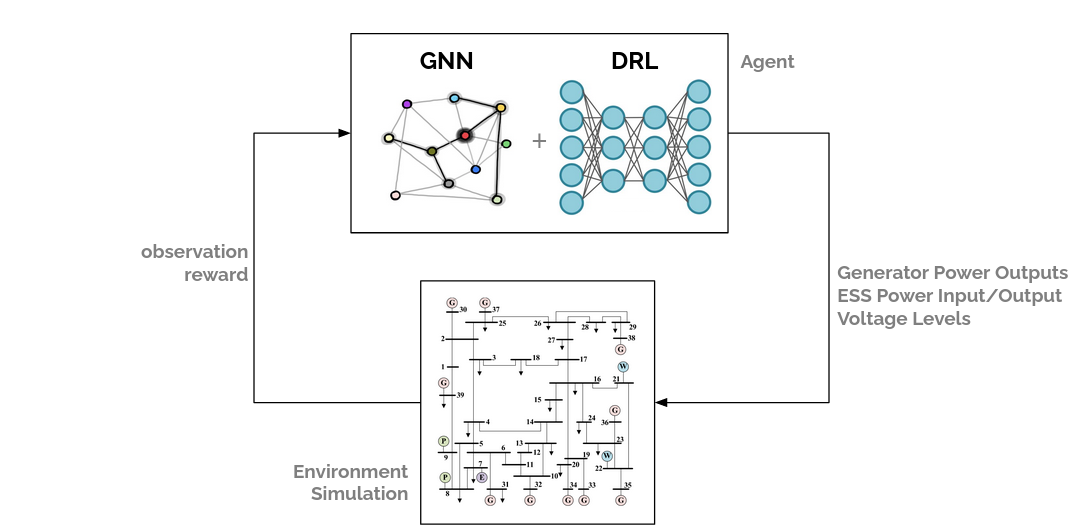
\includegraphics[width=0.85\linewidth]{./figures/arch.png}
	\caption{Solution Architecture}
	\label{fig:arch}
\end{figure}


To fulfil this, the agent adjusts the generator power output and voltage levels and manages the \ac{ESS} operation in real-time. \par
The solution is executed in the context of a power grid simulation that models the appropriate elements, properties, constraints and operating of the power distribution grid. This method is further described in the upcoming subsection \ref{sec:method}.



\section{Evaluation Metrics} \label{sec:eval-methods}

\begin{comment}
	* Sample Efficiency
	* Other methods
	* Equations
	* TODO
\end{comment}


The solution described in the previous subsections \ref{sec:arch} and \ref{sec:method} clearly involves intricate operational mechanisms, something that calls for a sophisticated evaluative process. Furthermore, given the comparative nature of this dissertation the evaluation and analysis methods will be key factors in studying and confronting the different combinations of \acp{GNN} and \ac{DRL}, as well as possible improvements in the integration of these techniques.
In this manner, we define the four dimensions for evaluating and analysing the different \ac{GRL} models:

\begin{description}
	\item[Learning efficiency] This dimension assesses how effectively the models learn and improve their decision-making process over time. It involves evaluating how quickly they converge to optimal or near-optimal dispatch strategies through the convergence rate. 
	
	\item[Computational Efficiency] It's crucial that the solution is able to perform well on real-time execution. In this context, not only it's important to assess the solution's decision computation performance but also to measure the time necessary for the model offline training, as well as the observed CPU/GPU resource utilization.
	
	\item[Dispatch Efficiency] The performance of the \ac{GRL} model in managing power distribution from the various generators will be mainly measured by the average operating cost (in \textit{Euros}) derived from the agent's sequence. Furthermore, other system behaviours will be analysed such as Renewable Energy Source Penetration, through the average ratio of maximum power and real power output, and \ac{ESS} utilization, through the average energy stored.
	
	\item[Scalability and Adaptation]  The solution will be applied to scenarios of several sizes for analysing its scalability. Furthermore, we will induce variations in the simulation scenarios to test the model's ability to handle topology changes.
\end{description}

\section{Work Plan} \label{sec:work-plan}


In order to make this project possible, we propose a 40-week work plan divided into four stages, whose start was in the last week of September 2023 and expected conclusion is scheduled for the last week of June 2024, observable in figure \ref{fig:gantt-chart}. 
The first stage, ranging from the first week of the plan to the delivery of this report, encompasses the \textbf{dissertation preparation} phase. This stage mainly addressed the initial knowledge acquisition necessary to understand this work's context and gather a basic grasp on the concepts and topics it addresses, namely:
\begin{itemize}
	 \item Reinforcement Learning
	\item Graph Theory
	\item Graph Representation Learning
	\item Graph Reinforcement Learning
	\item Graph Neural Networks
	\item Smart Grids Services
\end{itemize}
This process is followed by the analysis of existing research and approaches in \ac{GRL} and Smart Grid technologies which spans till the first week of January 2024, documented in chapter \ref{chap:literature-review}. Lastly, the preparation phase is also compromised of the PDIS report write-up until its delivery in the first week of February 2024, marking the end of this phase. \par
The preparation phase is followed by the \textbf{Development} phase. This stage encompasses all activities related to the system implementation, from the preparation of the simulation environment to the model training and calibration. The development phase spans from the first week of February 2024 to the second-to-last week of April 2024. \par
Next, the \textbf{Evaluation \& Analysis} stage is set, compromising the time frame where the various implemented models will be evaluated in the context of the previously mentioned dimensions and the evaluation results will be analysed. \par
Lastly, the \textbf{Dissertation} write-up and subsequent revision work will be performed, compromised of the write-up, proofreading and correction tasks and ranging from the end of the evaluation and analysis phase in the last week of April 2024 until the last week of the plan.


\begin{sidewaysfigure}
	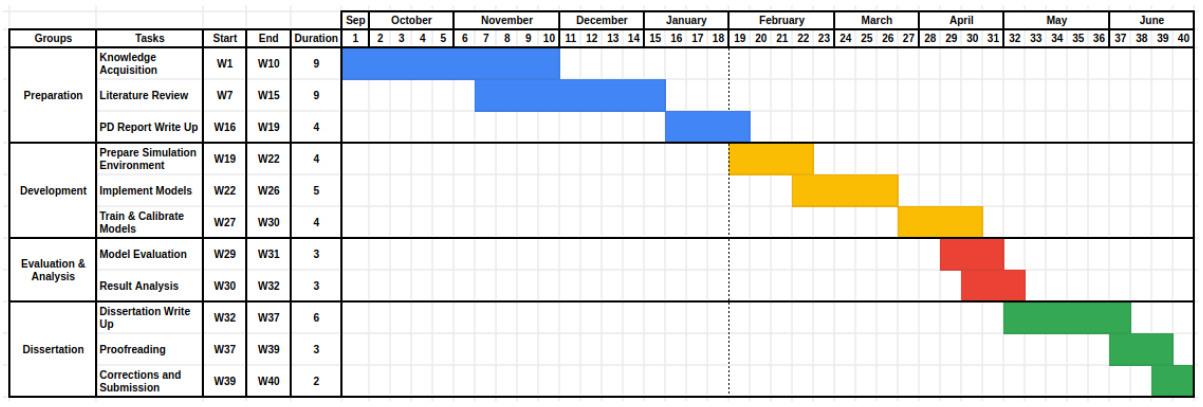
\includegraphics[width=1.0\linewidth]{./figures/gantt-chart.png}
	\caption{Project Work Plan}
	\label{fig:gantt-chart}
\end{sidewaysfigure}


%% !TeX spellcheck = en_GB
\chapter{Experimental Setup}

\begin{comment}
	* TODO
\end{comment}


\section{Simulation Environment}

Regarding the established methodology for enabling the implementation of the proposed solution, the \textit{grid2Op} framework \cite{rtefranceGrid2OpDocumentation} will be used for modelling the sequential decision-making process on simulated power distribution grid. \textit{grid2Op} is designed by RTE (\textit{Réseau de Transport d'Électricité}), the electricity transmission system operator of France, and is equipped with a variety of pre-defined scenarios used in coding competitions and based on real-world data \cite{rtefranceGrid2OpDocumentation}. This platform focuses on easing the job using the grid topology to control the power flows and also allowing for it to be reconfigured in real-time \cite{rtefranceGrid2OpDocumentation}. Additionally, enables to graphically plot the current observable state of the grid, as portrayed in figure \ref{fig:grid2op-graph}. Apart from graph topology, \textit{grid2op} also enables the manipulation of:

\begin{itemize}
	\item the \textbf{voltages} by manipulating the set-point value of the generators;
	\item the \textbf{active generation} by mapping the received observations to optimal sequences of dispatch actions \cite{rtefranceGrid2OpDocumentation}
\end{itemize}

This framework is compatible with the \textit{Gymnasium} framework \cite{faramafoundationGymnasiumDocumentation}, a widely used toolkit for developing \ac{RL} algorithms, which will also will be used in this work together with the Grid2Op simulation environment. 

\begin{figure}
	\centering
	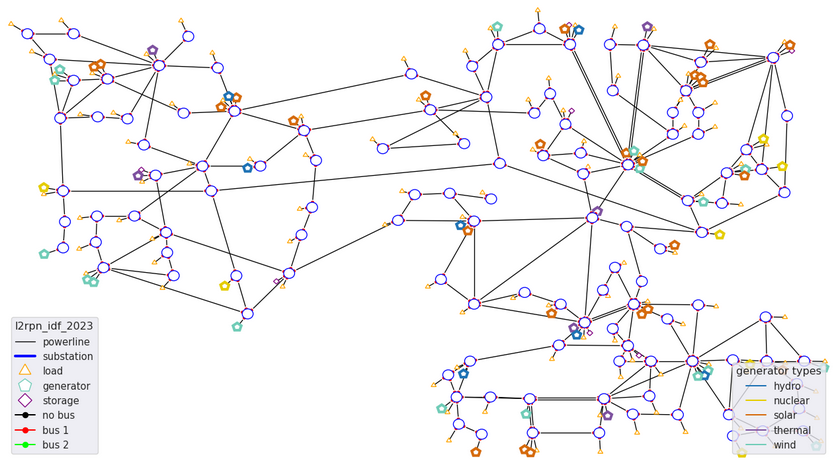
\includegraphics[width=0.85\linewidth]{./figures/grid2op-graph.png}
	\caption{Grid2Op \textit{l2rpn\_idf\_2023} 118-bus test case \cite{rtefranceGrid2OpDocumentation}}
	\label{fig:grid2op-graph}
\end{figure}

This platform focuses on describing the power distribution grids by modelling the following objects:
\begin{itemize}
	\item \textbf{Buses} are the fundamental objects of the power grid, representing nodes where power sources, loads and other elements are connected\cite{rtefranceGrid2OpDocumentation}.
	
	\item \textbf{Powerlines} represent edges in the power grid and connect the different buses together. They represent the physical transmission and distribution lines and allow power to flow from one part of the grid to another \cite{rtefranceGrid2OpDocumentation}.
	
	\item \textbf{Generators} are critical grid elements connected to buses whose main role is to produce power and maintain grid stability by balancing the energy supply and demand. They can be Conventional Thermal Generators, Wind Turbines or Photovoltaic Cells \cite{rtefranceGrid2OpDocumentation}.
	
	\item \textbf{Loads} consume power from the grid, simulating electricity use. They're also associated to an individual bus \cite{rtefranceGrid2OpDocumentation}.
	
	\item \textbf{Storage Units} can act as both consumers and producers. They're able to retain energy from the power grid when production surpasses demand for later injecting back power when convenient. Storage units are bound by a maximum energy storage capacity \cite{rtefranceGrid2OpDocumentation}.
\end{itemize}


Beyond \textit{grid2op} to build and run the test cases and \textit{gymnasium} as the RL framework, this project will use \textit{PyTorch} \cite{pytorchPyTorch} with \textit{PyTorch Geometric} \cite{pygteamPyGPytorch_geometric} library for developing the \ac{GNN} because of its extensive list of available implemented models. The different combinations of algorithms will be applied to a set of modified scenarios that fulfil the settled requirements. For Deep Reinforcement Learning algorithms, solutions with plain \ac{SAC}, \ac{DDPG} and \ac{PPO} approaches and combined with the \ac{GCN}, \ac{GAT} and \ac{GIN} architectures.  \par
Concerning result analysis, it's also important to point out the use of quantitative methods for evaluating the different implemented models, a topic that is further explored in the following section \ref{sec:eval-methods}.

\section{Scenarios}

\begin{table}[H] 
	\centering
	\caption{Test Case Sizes}
	\begin{tabular}{|P{2cm}|P{3.5cm}|P{3.5cm}|  }
		\hline
		& \textbf{l2rpn\_icaps\_2021} & \textbf{l2rpn\_idf\_2023} \\
		\hline
		\textbf{Buses} & 36 & 118 \\
		\hline
		\textbf{Powerlines} & 59  & 186  \\
		\hline
		\textbf{Generators} & 22 & 62  \\
		\hline
		\textbf{Loads} & 37 & 99 \\
		\hline
	\end{tabular}
	\label{tab:test-case}
\end{table}

This work will use the pre-defined \textit{grid2op} \textit{l2rpn\_icaps\_2021} and \textit{l2rpn\_idf\_2023} test environments, a modified case studies based on the original IEEE 118-bus system test case \cite{christiePowerSystemsTesta} of 36 and 118 buses, respectively. The first test case is a subset of the original 118-bus system with 50 years worth of data divided into independent \footnote{non-consecutive} weekly scenarios, while in the second case the system was modified to accommodate the \textit{possible energy mix} of France in 2035, containing 16 years of data \cite{rtefranceGrid2OpDocumentation}. The scenarios document the loads and productions at each time step, the grid layout (for display purposes), generator and \ac{ESS} characteristics \cite{rtefranceGrid2OpDocumentation} for a weekly episode, the sizes of test cases can be further observed in table \ref{tab:test-case}. In addition, the test cases data will be modified to reflect the defined requirements of this work. \par

\section{Experiments}

\subsection{GRL}

\subsection{DRL vs. GRL}

\subsection{Scalability}

\subsection{Adaptability}



\chapter{Result Discussion} \label{chap:results}
\begin{equation}
	\forall i \in N_\text{p}, \text{rho}_i (t_1) > \theta_\text{hard} \implies \forall t \in [t_1, t_1 + T_\text{reconnect}], F_i (t) = 0
\end{equation}

\begin{equation}
	\forall i \in N_\text{p}, t \in [t_1, t_1 + T_\text{soft}], \text{rho}_i (t) > \theta_\text{soft} \implies \forall t \in [t_1 + T_\text{soft}, t + T_\text{reconnect}], F_i (t)= 0
\end{equation}
In this chapter, the obtained results are thoroughly analysed and discussed. The performed experiments can be subdivided into 6 categories: Curtail Lower Limit (section \ref{sec:results-lower}), Limit Infeasible Curtailment Actions \ref{sec:results-limit}, Reward Tests \ref{sec:results-rewards}, \acp{GNN} Hyperparameter Tuning, \ac{GNN} Implementation Comparison \ref{sec:results-gnn-comp} and Scability Tests \ref{sec:results-scalability}.

\section{Implementation Details} \label{sec:results-implementation}

The development of \ac{GRL} algorithms posed as a complex and difficult problem. As mentioned in the literature review and restated in the problem statement, there is a scarse availability of open-source implementations and frameworks that are implemented to accommodate the implementation of these techniques. 

\subsection{Reproducibility}

A major concern and challenge brought with the technologies at hand was to implement a solution that brought reproducible results. This is critical to ensure appropriate analysis and calibration of the model as well as to allow other academics and interested readers to reproduce the results and follow the tuning process. \par

Initially, exploratory experiments with \textit{stable-baselines3} revealed that the \ac{DRL} algorithms were developed in a deterministic and reproducible nature but with the inclusion of the \textit{torch\_geometric}  \acp{GNN} the results were not consistent. \par

In this context, the documentation of both libraries were thoroughly analysed and studied and it was ensured that all of the appropriate seeds were being defined. However, results in the same machine still differed. This was later found to be related with the non-deterministic nature of some \textit{torch\_geometric} functions in the GPU, namely \textit{torch-scatter} operations \cite{NotReproducibleSetting} \cite{ReproducibilityPyTorchDocumentation}. \par

Although, at first, this issue seemed unsolvable, a specific parameter was found in the \textit{PyTorch} Documentation \cite{ReproducibilityPyTorchDocumentation} that successfully mitigated this problem and allowed for result reproducibility. Nevertheless, for different machines, the results still showed inconsistencies. \par

\begin{lstlisting}
	import torch
	torch.use_deterministic_algorithms(True)
\end{lstlisting}

\subsection{Flexibility}

One of the objectives that was also a large focus of the implemented solution, was to allow different combinations of \ac{DRL} and \ac{GNN} algorithms. Since \ac{GRL} still is a relatively recent field, it's important that research around this area builds foundations for other studies and this is facilitated with the developed flexible framework that enables experiments on other models that are currently unexplored. \par
With the advantages of having two popular frameworks for each type of algorithms with a consistent API for both made this goal easier to achieve than the former one associated with reproducibility. \par


\section{Reward Function} \label{sec:results-rewards}

Several implementations posed as relevant formulas to describe the reward function of the environment, namely three: Economic Reward, \acp{RES} Penalty Factor Reward and \acp{RES} Bonus Reward. The first considered only the saved cost in non-renewable generators operation, while the second and third accounted for \ac{RES} maximization in a penalty and bonus factor, respectively.
\par
Considering the new parameter introduced by both the Penalty and Bonus Factor rewards, $\beta$, the experiments took into account three distinct values: $\{0.4, 0.6, 0.8\}$.  \par
It's important to note that when evaluating and comparing reward functions, the average cumulative reward values retain different meanings. Furthermore, although still relevant to analyse the convergence of the models, other metrics were favoured, such as daily operating cost, abandoned \ac{RES} energy and the survival rate. \par

\begin{figure}[H]
	\centering
	\subfloat{}{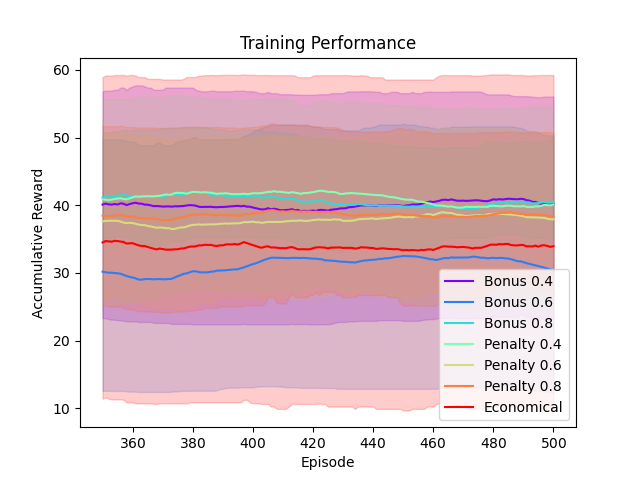
\includegraphics[width=.45\textwidth]{graphs/reward/training_performance.png}}
	\hskip1ex
	\subfloat{}{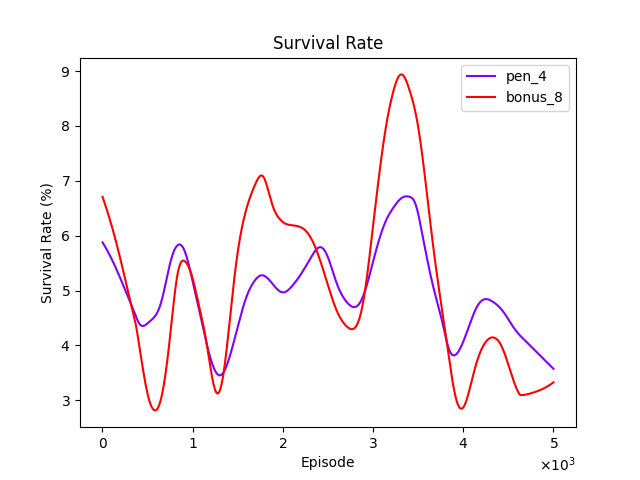
\includegraphics[width=.45\textwidth]{graphs/reward/survival_rate.png}} 
	\vfill
	\subfloat{}{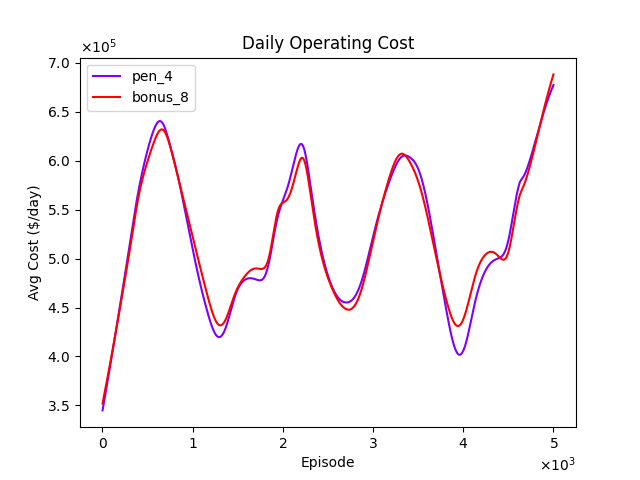
\includegraphics[width=.45\textwidth]{graphs/reward/daily_cost.png}} \hskip1ex
	\subfloat{}{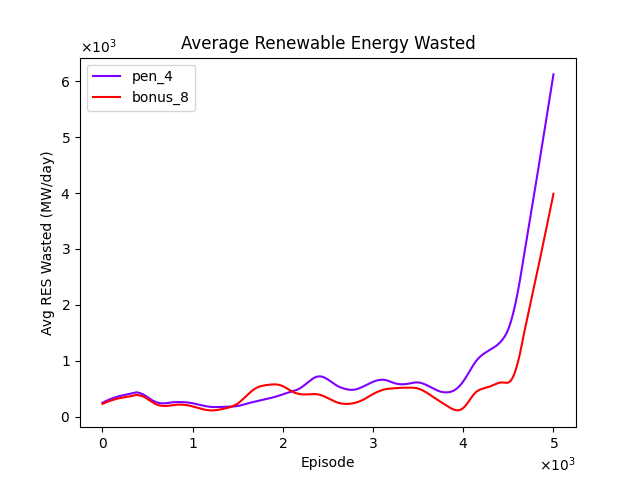
\includegraphics[width=.45\textwidth]{graphs/reward/res_wasted.png}} 
	\caption{Training Results of the Experiments concerning Observation Space.}
	\label{fig:train-reward}
\end{figure}

  \begin{table}[h!]
	\centering
	\caption{Test Results for Reward Parameters Experiments}
	\begin{tabular}{cccccc}
		\toprule
		\multirow{2}{*}{\textbf{reward}} & \multirow{2}{*}{\textbf{$\beta$}} & \multicolumn{4}{c}{\textbf{Metrics}} \\ 
		\cmidrule(lr){3-6}
		&  & \textbf{Avg. CR} & \textbf{Avg. Length} & \textbf{Avg. DOC} & \textbf{Avg. REW} \\ 
		\midrule
		bonus & 0.8 & 40.88 & 96.43 & 560927.60 & 3115.18 \\
		penalty & 0.4 & 40.57 & 80.75 & 565893.63 & 4100.20 \\
		bonus & 0.4 & 40.13 & 76.23 & 565757.16 & 3723.72  \\
		penalty & 0.8 & 38.22 & 76.35 & 555582.14 & 2612.34 \\
		penalty & 0.6 & 37.54 & 81.40 & 558362.82 & 2570.71 \\
		economical & - & 34.38 & 58.65 & 574981.17 & 2610.70 \\
		bonus & 0.6 & 30.78 & 55.06 & 566786.07 & 2750.34 \\
		% Add more rows as needed
		\bottomrule
	\end{tabular}
	\label{tab:test-reward}
\end{table}


\par
Results revealed that the proposed implementations were superior to the already defined Economic Reward both in survivability and overall performance of the models. The with the best results were observed in the Bonus Factor Reward with $\beta = 0.4$. Although





\begin{comment}
	* Best SAC and GNN parameters
	* Explain that SAC was used for most experiments as a baseline
\end{comment}

\section{Observation Space} \label{sec:results-obs}

Regarding the observation space, two matters were found to be worth to analyse. 
Firstly, it was hypothesized that using time keys (minute, hour, and day of the week) instead of the current step might help the model find temporal patterns in the sequential process that could yield performance improvements. \par
Additionally, given the complexity of the problem at hand, a min-max scale was applied in particular keys also with the goal of increasing learning efficency and overall performance. The scaling was applied to $P^\text{NRES}_i (t)$, $P^\text{RES}_i (t)$, and $\overline{P^\text{RES}_i} (t)$. \par

\begin{equation}
	x' = \frac{x - \min x}{\max x - \min x}
\end{equation}

  \begin{table}[h!]
	\centering
	\caption{Test Results for Observation Space Parameters Experiments}
	\begin{tabular}{cccccc}
		\toprule
		\multirow{2}{*}{\textbf{step}} & \multirow{2}{*}{\textbf{scaled}} & \multicolumn{4}{c}{\textbf{Metrics}} \\ 
		\cmidrule(lr){3-6}
		& & \textbf{Avg. CR} & \textbf{Avg. Length} & \textbf{Avg. DOC} & \textbf{Avg. REW} \\ 
		\midrule
		
		True & False & 40.00 & 65.26 & 559046.91 & 2302.77 \\
		False & False  & 56.31 & 85.65 & 565029.79 & 2088.03 \\
		True & True & 39.93 & 66.036 & 567707.16  & 2581.26 \\
		False & True & 45.33 & 69.96 & 552337.96 & 2520.84 \\
		% Add more rows as needed
		\bottomrule
	\end{tabular}
	\label{tab:test-obs}
\end{table}


\section{Action Space} \label{sec:results-action}

The initial exploratory experiments and posterior training performance analysis showed significant instability and lack of convergence of \ac{DRL} models. During the experimentation phase, the developed implementations, SAC and GCN-SAC, showed a significantly reduced survival rate. This posed a substantial problem since models failed to survive enough steps to appropriately learn economic policies, leading to relatively short results in their test phase. \par

\begin{table}[h!]
	\centering
	\caption{Test Results for \texttt{no\_curtail} Environment Parameter Search}
	\begin{tabular}{ccccc}
		\toprule
		\multirow{2}{*}{\textbf{no\_curtail}} & \multicolumn{4}{c}{\textbf{Metrics}} \\ 
		\cmidrule(lr){2-5}
		&  \textbf{Avg. CR} & \textbf{Avg. Length} & \textbf{Avg. DOC} & \textbf{Avg. REW} \\ 
		\midrule
		True & 130.15 & 676.74 & 536423.98 & 0.0 \\
		False & 22.13 & 37.14 & 619721.30  & 10315.47  \\
		% Add more rows as needed
		\bottomrule
	\end{tabular}
	\label{tab:test-curtail}
\end{table}

Upon further research, the root of this problem was found to be related to the inclusion of curtailment actions, which made the action space more complex and, in turn, severely affected the models' performance. Table \ref{tab:test-curtail} clearly states this problem, by highlighting the test results of two models with and without curtailment actions. As observed, the inclusion of curtailment actions caused an average cumulative reward decrease of 83.00\% in relation to the model without these type of actions. Additionally, the survivability of the worst model was also significantly inferior, with an average episode length of 37.14 steps. \par
It was found that during the exploratory phase, the abrupt changes in curtailment caused infeasible states of the system and, consequently, an early episode truncation. This caused the model to perform very poorly and, as a consequence, severely affected the learning efficiency, since the algorithms were not managing to survive enough steps to appropriately learn optimal dispatch policies. \par
With the purpose of further analysing and solving this problem, two methods described in the following subsections \ref{sec:results-limit} and \ref{sec:results-lower} were experimented to mitigate it.


\subsection{Limit Curtailment Infeasible States} \label{sec:results-limit}

The first method that was analysing the effect of using the grid2op  \texttt{LIMIT\_INFEASIBLE\_CURTAILMENT\_STORAGE\_ACTION} parameter, which according to its own long name and documentation limits infeasible system states derivative from curtailment (and storage) actions. \par
For this purpose, another model was trained with this flag set to \texttt{True}. 

\begin{comment}
	TODO -> LIMIT Experiements Graphs and tables
\end{comment}



The training results confirmed the initial suspicions, demonstrating that while performance is significantly and negatively affected when curtailment actions are included, by setting the \texttt{LIMIT\_INFEASIBLE\_CURTAILMENT\_STORAGE\_ACTION} the model was able to achieve higher results than without the parameter. As observed in table \ref{tab:test-limit}, the usage of the parameter translated into an improvement of 346.63 \% in average cumulative reward and 1100.02 \% in survival rate compared with the worst model. \par

\begin{comment}

\begin{figure}[H]
	\centering
	\subfloat{}{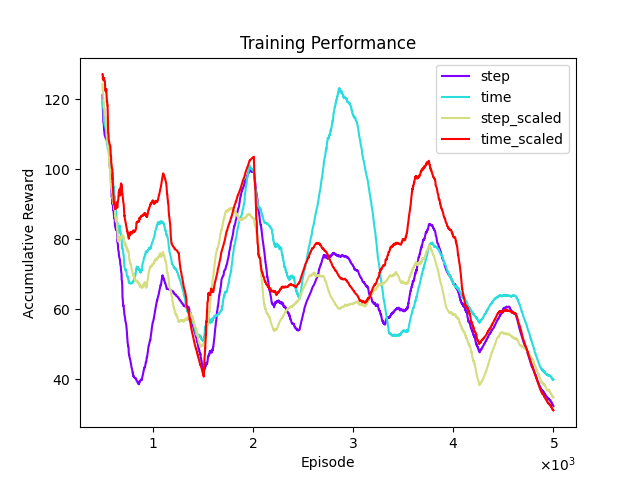
\includegraphics[width=.45\textwidth]{graphs/obs/training_performance.png}}
	\hskip1ex
	\subfloat{}{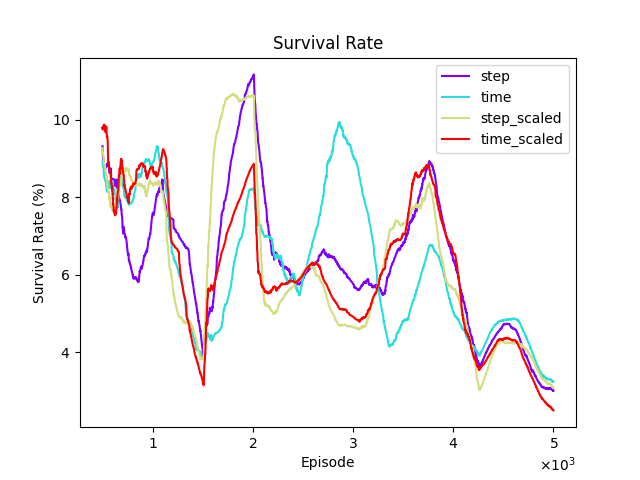
\includegraphics[width=.45\textwidth]{graphs/obs/survival_rate.png}} 
	\vfill
	\subfloat{}{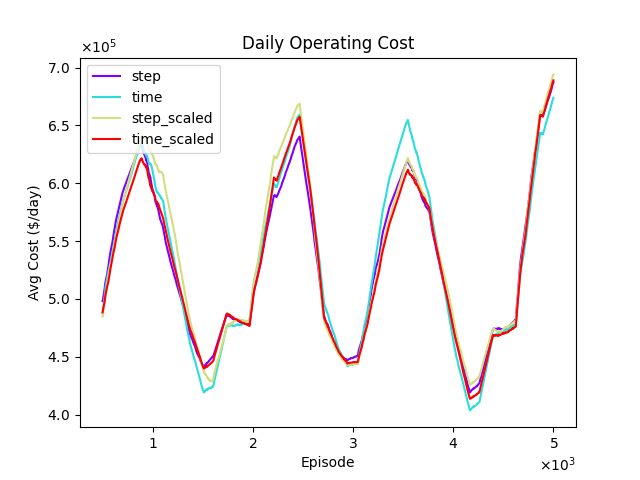
\includegraphics[width=.45\textwidth]{graphs/obs/daily_cost.png}} \hskip1ex
	\subfloat{}{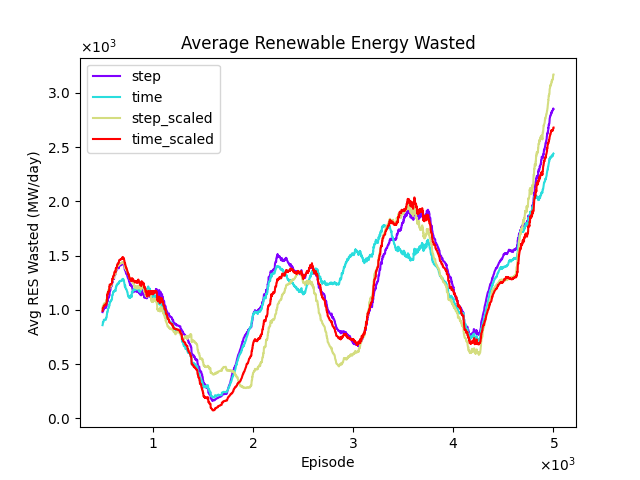
\includegraphics[width=.45\textwidth]{graphs/obs/res_wasted.png}} 
	\caption{Training Results of the Experiments concerning Observation Space.}
	\label{fig:train-obs}
\end{figure}
	
\end{comment}

\begin{table}[h!]
	\centering
	\caption{Test Results for \texttt{limit\_inf} \textit{Grid2Op} Parameter Experiments}
	\begin{tabular}{cccccc}
		\toprule
		\multirow{2}{*}{\textbf{no\_curtail}} & \multirow{2}{*}{\textbf{limit\_inf}} & \multicolumn{4}{c}{\textbf{Metrics}} \\ 
		\cmidrule(lr){3-6}
		&  & \textbf{Avg. CR} & \textbf{Avg. Length} & \textbf{Avg. DOC} & \textbf{Avg. REW} \\ 
		\midrule
		True & False & 130.15 & 676.74 & 536423.98 & 0.00 \\
		False & True  & 98.84 & 445.77 & 588610.57 & 8039.41 \\
		False & False & 22.13 & 37.14 & 619721.30 & 10315.47 \\
		
		% Add more rows as needed
		\bottomrule
	\end{tabular}
	\label{tab:test-gcn-limit}
\end{table}

Although its usage has an apparent positive effect on model performance, it still did not mitigate the concerns related to the introduced complexity of curtailment actions. The model without these actions still outperformed the others by a large margin, outlining a difference of 31.31 reward units on average to the second-best model. The proposed method failed to mitigate the advantage brought by the behaviour of the model without curtailment actions, which by default uses all of the available renewable energy at each timestep, resulting in 0.0 MW of wasted \ac{RES} energy.

\subsection{Curtailment Lower Limit} \label{sec:results-lower}

Another possible solution to the problem of added intricacy advent from including curtailment actions is the definition of a lower bound for curtailment actions that restricts the model operation in this regard. \par

\begin{equation} \label{eq:linear-decay}
	y = 1 - \frac{(1 - \underline{P^\text{RES}}) E_\text{train}}{E_\text{decay\_end}}
\end{equation}

\begin{equation} \label{eq:sqrt-decay}
	y = (1 - \underline{P^\text{RES}}) \sqrt[\alpha]{\frac{E_\text{decay\_end} - E_\text{train}}{E_\text{train}}}
\end{equation}

Reflecting on the secondary goal of maximising the usage of generated renewable energy, the idealisation of a lower limit to confine the curtailment action space became a feasible solution to aid in the model's learning efficiency. In this manner, this condition was included in the implementation along with three possible strategies applied solely in the training stage:
\begin{itemize}
	\item Fixed lower bound
	\item Linear decreasing lower bound
	\item Square Root decreasing lower bound
\end{itemize}


An experiment compared the performance of the proposed strategies and the impact of this method on the former one introduced in subsection \ref{sec:results-limit}. The test results are observable in table \ref{tab:test-decay}.

\begin{table}[h!]
	\centering
	\caption{Test Results for \texttt{decay\_type} \ac{GCN} Parameter Experiments}
	\begin{tabular}{ccccc}
		\toprule
		  \multirow{2}{*}{\textbf{decay}} & \multicolumn{4}{c}{\textbf{Metrics}} \\ 
		\cmidrule(lr){2-5}
		& \textbf{Avg. CR} & \textbf{Avg. Length} & \textbf{Avg. DOC} & \textbf{Avg. REW} \\ 
		\midrule
		sqrt & 153.77 & 628.19 & 579978.88 & 7356.86 \\
		fixed & 122.58 & 461.28 & 541391.22 & 7480.09 \\
		linear & 111.52 & 289.36 & 550832.62 & 7092.56 \\
		None & 98.84 & 445.77 & 588610.57 & 8039.41 \\
		% Add more rows as needed
		\bottomrule
	\end{tabular}
	\label{tab:test-decay}
\end{table}

Results proved that the introduced curtailment lower bounds considerably increased the model's training performance and convergence, with the square root decay method achieving the overall highest average cumulative reward during the test phase. The models with a fixed lower bound and linear decay also exceeded the method presented in the former subsection without outperforming the model without curtailment. The best model outperformed the one without curtailment actions in average cumulative reward by 18.15 \%, which showed the relevance of including these actions to learning efficiency and justified their usage.\par
Nevertheless, the model with no curtailment reached a slightly higher survival rate without curtailment actions, as observable in table \ref{tab:test-curtail-comp}.


\begin{table}[h!]
	\centering
	\caption{Test Results for \texttt{decay\_type} \ac{GCN} Parameter Experiments}
	\begin{tabular}{ccccccc}
		\toprule
		\multirow{2}{*}{\textbf{no\_curtail}} & \multirow{2}{*}{\textbf{limit\_inf}} & \multirow{2}{*}{\textbf{decay}} & \multicolumn{4}{c}{\textbf{Metrics}} \\ 
		\cmidrule(lr){4-7}
		&  & & \textbf{Avg. CR} & \textbf{Avg. Length} & \textbf{Avg. DOC} & \textbf{Avg. REW} \\ 
		\midrule
		False & True & sqrt & 153.77 & 628.19 & 579978.88 & 7356.86 \\
		False & False & sqrt & 153.77 & 628.19 & 579978.88 & 7356.86 \\
		True & False & None & 130.15 & 676.74 & 536423.98 & 0.00 \\
		False & True & None & 98.84 & 445.77 & 588610.57 & 8039.41 \\
		False & False & None &  22.13 & 37.14 & 619721.30 & 10315.47 \\
		
		% Add more rows as needed
		\bottomrule
	\end{tabular}
	\label{tab:test-curtail-comp}
\end{table}


Interestingly, the combination of both proposed methods had no performance improvement, with the most significant being observed in the lower bound method. This clearly shows the superiority of this solution over the other, which, on its own, did not justify the usage of curtailment actions. However, given that the usage of the \texttt{LIMIT\_INFEASIBLE\_CURTAILMENT\_STORAGE\_ACTION} parameter also had a positive effect on performance and the author was not sure that the simultaneous usage of both methods always translated into the same learning efficiency as using only the lower bound method, a combination of both solutions was considered as the optimal procedure.

\section{\acp{GNN} Hyperparameter Tuning} \label{sec:results-gnn}

As a key area of this research work, the \ac{GNN} component of the proposed algorithm was given a special emphasis on what accounts for hyperparameter tuning. Concrete experiments were devised to assess the performance of different parameter combinations, mainly focusing on the \ac{GCN} architecture. This section is organised as follows: in this first subsection \ref{sec:results-aggr}, the performance of the several available aggregation schemes is unveiled and analysed; in subsection \ref{sec:results-layers} the focus is shifted towards the number of \ac{GNN} layers; in the following subsection \ref{sec:results-gcn-param} the effect of other specific \ac{GCN} parameters is analysed, and, lastly, in the last subsection \ref{sec:results-gat-param} the same process is performed for the \ac{GAT} architecture. \par 


\subsection{Aggregate Function} \label{sec:results-aggr}

The aggregation function is a crucial component of \ac{GNN} algorithms, and because of this fact, it was the first parameter investigated. An experiment was conducted to ascertain the best-performing aggregation function of the \ac{GCN} architecture, and the available schemes include the following:
\begin{itemize}
	\item \texttt{sum}
	\item \texttt{max}
	\item \texttt{min}
	\item \texttt{mean}
	\item \texttt{mul}
\end{itemize}

\begin{figure}[ht]
	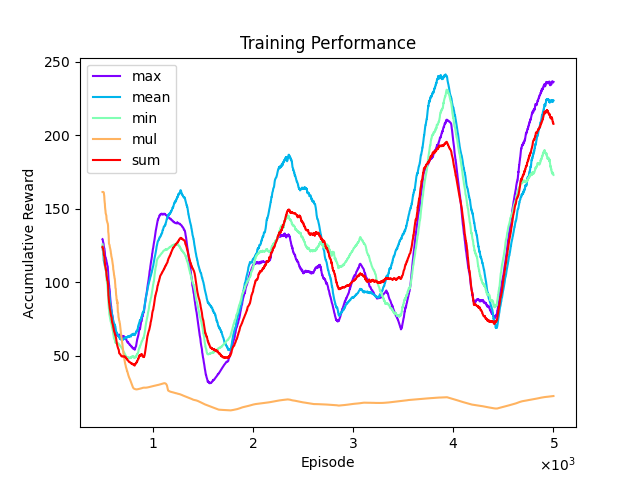
\includegraphics[width=0.75\textwidth]{graphs/aggr/training_performance.png}
	\caption{Training Performance per Aggregation Scheme}
	\label{fig:train-perf-aggr}
\end{figure}

As observed in figure \ref{fig:train-perf-aggr}, training performance  only revealed an apparently poor performing multiplication scheme, with other schemes achieving somewhat similar results. However, this aggregation function ended up achieving a significantly higher survival rate during training, which is verified in the test results depicted in table \ref{tab:test-aggr}. \par

\begin{figure}[ht]
	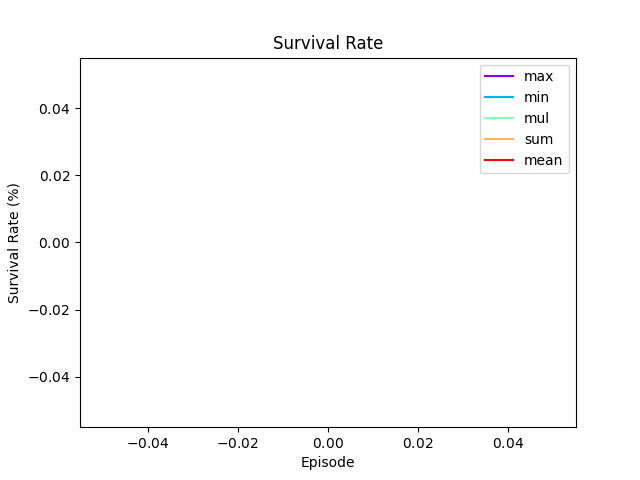
\includegraphics[width=0.75\textwidth]{graphs/aggr/survival_rate.png}
	\caption{Survival Rate per Aggregation Scheme}
	\label{fig:train-surv-aggr}
\end{figure}

As observed in figure \ref{fig:train-perf-aggr}, training performance revealed a poorly performing multiplication scheme compared to the other tested functions. However, the multiplication function yielded a significantly high average length of 1104.06 in tests, over 43\% of the model with the second-best survivability (sum), while at the same time achieving only 15.76 of average cumulative reward, which is a significantly lower value compared with the model with the second-to-last reward of 80.89. As observed in the test results, this case is primarily due to a high average daily operating cost, close to four thousand euros more than any other model. Beyond that, this model did not perform optimally when analysing the average energy from \ac{RES} wasted, with over three thousand megawatts of unused renewables in relation to every other model. \par

\begin{table}[h!]
	\centering
	\caption{Test Results for \texttt{aggr} \ac{GCN} Aggregation Function Experiments}
	\begin{tabular}{ccccc}
		\toprule
		\multirow{2}{*}{\textbf{aggr}} & \multicolumn{4}{c}{\textbf{Metrics}} \\ 
		\cmidrule(lr){2-5}
		&  \textbf{Avg. CR} & \textbf{Avg. Length} & \textbf{Avg. DOC} & \textbf{Avg. REW} \\ 
		\midrule
		max & 119.16 & 677.75 & 560219.45 & 6564.49 \\
		sum & 114.58 & 768.58 & 569952.37 & 7268.28 \\
		mean & 92.90 &  551.24 & 557637.84 & 6268.06 \\
		min & 80.89 & 495.70 & 559033.63 & 6687.94 \\
		mul & 15.76 & 1104.06 & 608319.66 & 10305.96 \\
		% Add more rows as needed
		\bottomrule
	\end{tabular}
	\label{tab:test-gcn-aggr}
\end{table}


The test results also showed that the function with the best average cumulative reward was \texttt{max}, outperforming the second-placed \texttt{sum} by almost five reward points. Furthermore, this model managed to do better than average in most metrics while simultaneously being outperformed in all of them. This shows the balance between the importance of cost saving, the maximisation of renewable energy and model survivability that the algorithm must equate for optimally solving the problem of \ac{DED}. \par
In this manner, although the \textit{max} function yielded the best performance only by a small margin, the author still chose it as the optimal aggregation scheme.

\begin{comment}
	TODO ->>> TOTAL TIME
\end{comment}

\subsection{Layers} \label{sec:results-layers}

Another critical characteristic of \ac{GNN} architecture is the number of layers. Another separate experiment was devised to assess the optimal value for this parameter, considering the \texttt{max} aggregation scheme, which, as exposed in the last subsection \ref{sec:results-aggr}, yielded the best results. The models had one to six \ac{GCN} layers, and the results are observable in table \ref{tab:test-layers}.

\begin{figure}[H]
	\centering
	\subfloat{}{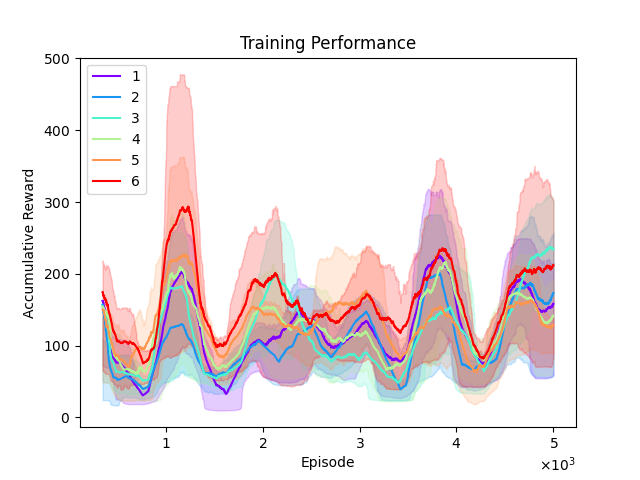
\includegraphics[width=.45\textwidth]{graphs/layers/training_performance.png}}
	\hskip1ex
	\subfloat{}{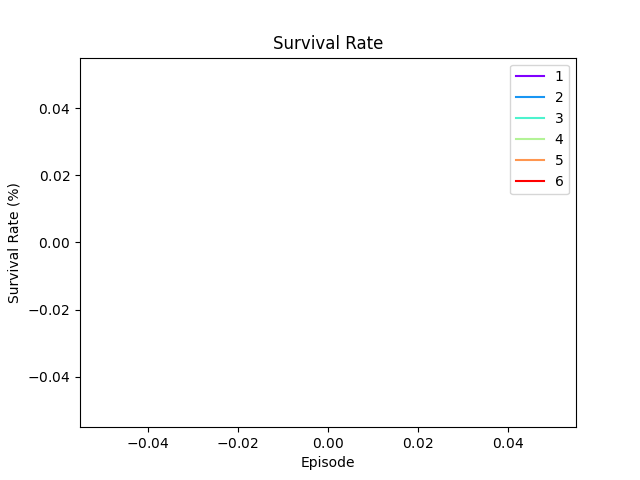
\includegraphics[width=.45\textwidth]{graphs/layers/survival_rate.png}} 
	\vfill
	\subfloat{}{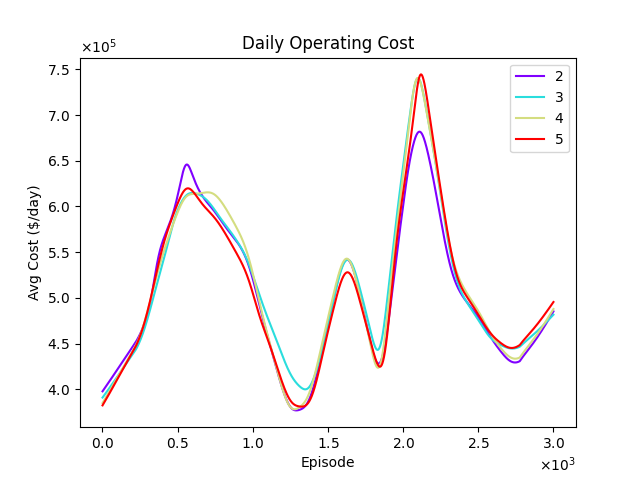
\includegraphics[width=.45\textwidth]{graphs/layers/daily_cost.png}} \hskip1ex
	\subfloat{}{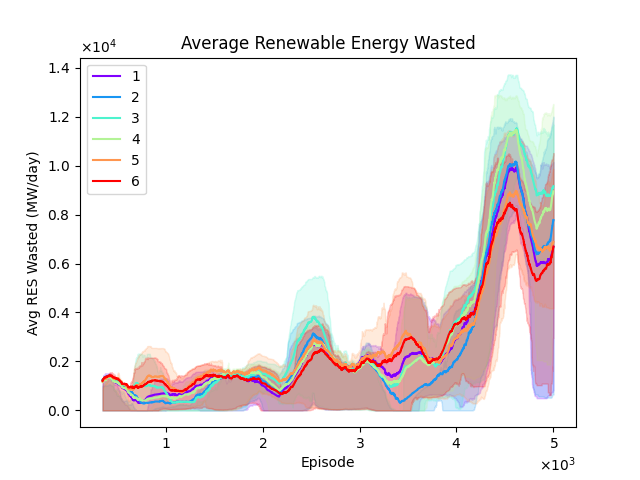
\includegraphics[width=.45\textwidth]{graphs/layers/res_wasted.png}} 
	\caption{Training Results of models with 1, 2, 3, 4, 5, and 6 \ac{GNN} Layers}
	\label{fig:train-layers}
\end{figure}

Regarding the study conducted around this \ac{GNN} characteristic, a configuration of six layers stands out from the rest, reaching an average cumulative reward of 135.75 reward units. This value represents a 13.92\% improvement regarding the second-best model in this metric, which was the one-layer network.

  \begin{table}[h!]
	\centering
	\caption{Test Results for \texttt{num\_layers} \ac{GCN} Parameter Experiments}
	\begin{tabular}{ccccc}
		\toprule
		\multirow{2}{*}{\textbf{num\_layers}} & \multicolumn{4}{c}{\textbf{Metrics}} \\ 
		\cmidrule(lr){2-5}
		&  \textbf{Avg. CR} & \textbf{Avg. Length} & \textbf{Avg. DOC} & \textbf{Avg. REW} \\ 
		\midrule
		
		6 & 135.75 & 487.09 & 560147.77 & 5862.49 \\
		1 & 119.16 & 677.75 & 560219.45 & 6564.49 \\
		3 & 110.73 & 736.32 & 567510.58 & 7116.24 \\
		4 & 98.67 & 451.51 & 577464.90 & 8641.05 \\
		5 & 92.97 & 286.65 & 550205.21 & 6397.41 \\
		2 & 91.58 & 694.67 & 575093.64 & 5989.95 \\
		% Add more rows as needed
		\bottomrule
	\end{tabular}
	\label{tab:test-layers}
\end{table}

Generally, the calibration process has failed to reach ideal levels of survivability.
Once again, the top-performing model in cumulative performance did not correspond to the best metric, the three-layered network, with an average survival rate of 36.52\%. This value corresponds to an average survivability of 2.56 days per weekly episode, which, in a real-world scenario, models would break the power grid constraints after only a few days of operation. 

\subsection{Output Features} \label{sec:results-out}
 
  \begin{table}[h!]
	\centering
	\caption{Test Results for \texttt{out\_channels} \ac{GCN} Parameter Experiments}
	\begin{tabular}{ccccc}
		\toprule
		\multirow{2}{*}{\textbf{out\_channels}} & \multicolumn{4}{c}{\textbf{Metrics}} \\ 
		\cmidrule(lr){2-5}
		&  \textbf{Avg. CR} & \textbf{Avg. Length} & \textbf{Avg. DOC} & \textbf{Avg. REW} \\ 
		\midrule
		6 & 135.75 & 487.09 & 560147.77 & 5862.49 \\
		36 & 95.92 & 571.48 & 582984.75 & 7575.34 \\
		18 & 88.47 & 777.78 & 562226.73 & 6874.71 \\
		3 & 87.68 & 428.30 & 563134.93 & 9497.97 \\
		% Add more rows as needed
		\bottomrule
	\end{tabular}
	\label{tab:test-gcn-out}
\end{table}

\subsection{\ac{GCN} Parameters} \label{sec:results-gcn-param}

Some particular \ac{GNN} parameters not covered in the last subsections were also deemed relevant to analyse. This examination was motivated by an exploratory investigation that revealed the potential performance increase of using these parameters. \par
The \texttt{act\_first} parameter controls if the \ac{GNN} activation function, which is ReLU, is applied before the computation of the symmetric normalisation coefficients. The other parameter analysed was the \texttt{improved} flag, which defines whether the model computes $mathbf{\hat{A}}$ as $\mathbf{A} + 2\mathbf{I}$. \par
In this context, a grid search was conducted around these two parameters, whose test results are observable in table \ref{tab:test-gcn-params}.
 
 \begin{figure}[H]
 	\centering
 	\subfloat{}{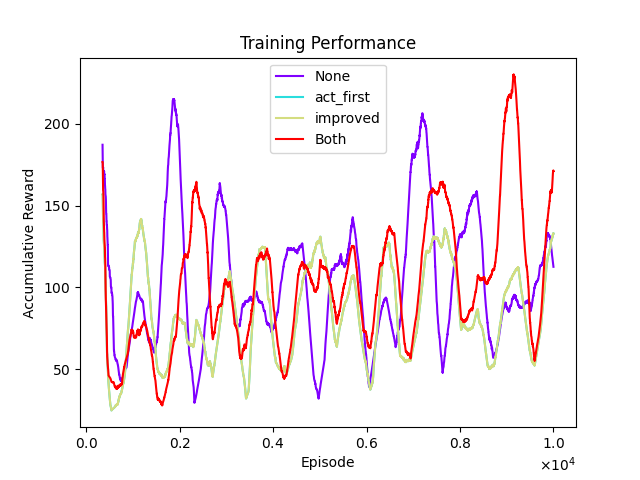
\includegraphics[width=.45\textwidth]{graphs/gcn_param/training_performance.png}}
 	\hskip1ex
 	\subfloat{}{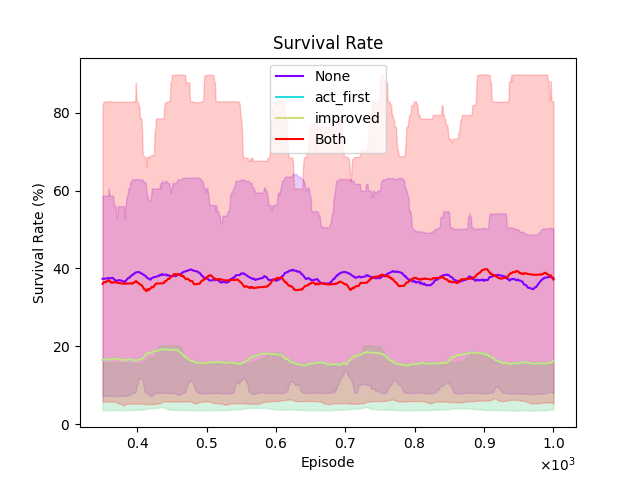
\includegraphics[width=.45\textwidth]{graphs/gcn_param/survival_rate.png}} 
 	\vfill
 	\subfloat{}{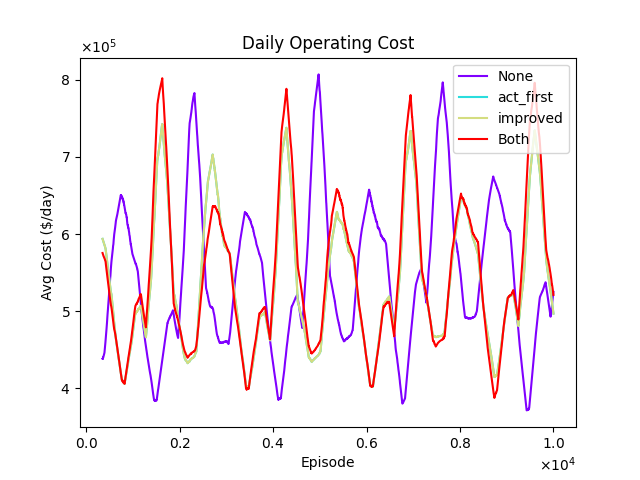
\includegraphics[width=.45\textwidth]{graphs/gcn_param/daily_cost.png}} \hskip1ex
 	\subfloat{}{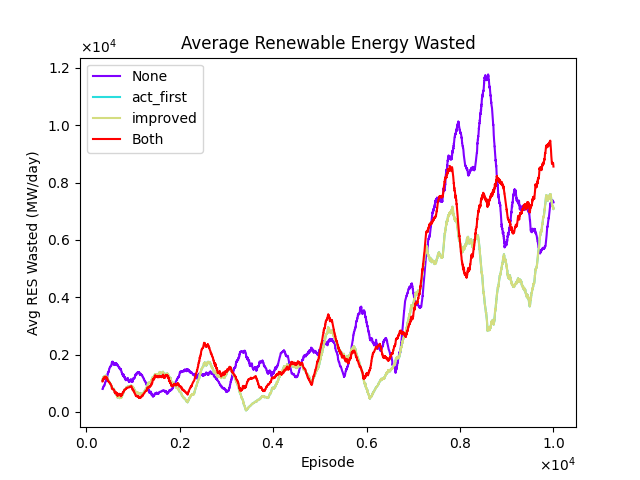
\includegraphics[width=.45\textwidth]{graphs/gcn_param/res_wasted.png}} 
 	\caption{Training Results of models with 2, 3, 4 and 5 \ac{GNN} Layers}
 	\label{fig:train-gcn-param}
 
 \end{figure}
 
 
 
  \begin{table}[h!]
 	\centering
 	\caption{Test Results for \texttt{act\_first} and \texttt{improved} \ac{GCN} Parameter Search}
 	\begin{tabular}{cccccc}
 		\toprule
 		\multirow{2}{*}{\textbf{act\_first}} & \multirow{2}{*}{\textbf{improved}} & \multicolumn{4}{c}{\textbf{Metrics}} \\ 
 		\cmidrule(lr){3-6}
 		&  &  \textbf{Avg. CR} & \textbf{Avg. Length} & \textbf{Avg. DOC} & \textbf{Avg. REW} \\ 
 		\midrule
 		True & False & 118.97 & 640.40 & 564201.23 & 7167.22 \\
 		True & True & 101.26 & 738.60 & 546592.78 & 6297.46 \\
 		False & False & 78.62 & 759.82 & 575798.57& 7640.76 \\
 		False & True & 75.29 & 328.78 & 548378.53 & 5043.04 \\
 		% Add more rows as needed
 		\bottomrule
 	\end{tabular}
 	\label{tab:test-gcn-params}
 \end{table}
 
 
 The use of \texttt{act\_first} positively affected performance, considering the two best results. In contrast, the models that performed the activation after normalisation failed to surpass 100 reward units. Furthermore, the models benefited from not defining \texttt{improved}, translating into a cumulative reward improvement in both cases. In this manner, the chosen optimal configurations for these parameters were \texttt{act\_first = True} and \texttt{improved = False}, corresponding to the combination used for the best-performing model.
 
\subsection{\ac{GAT} Parameters} \label{sec:results-gat-param}
 
As another prominent state-of-the-art architecture, the \ac{GAT} network was also target to some tuning in specific parameters. This seemed appropriate given the tuning process the \ac{GCN} network was particularly subject to, intending to also leverage the specific attributes of the \ac{GAT} architecture. The optimal combination of \texttt{aggr}, \texttt{num\_layers}, and \texttt{out\_channels} observable for the \ac{GCN} model was reused in this architecture. While this was not an optimal approach, this decision was taken given the timing constraints of the project and the often significant amount of training time. \par

In this manner, an experiment was conducted around the three most relevant parameters of this model: \texttt{act\_first}, \texttt{heads} and \texttt{v2}. The first, as seen in the previous subsection, positively affected the model's test results and learning efficiency, which encouraged further analysis. \par

The second and third parameters are specific to the \ac{GAT} network, with the first representing the number of attention heads used in the model and the second consisting of a flag that controls the use of the GATv2 architecture proposed in \cite{brodyHowAttentiveAre2022}. \par

This study used a random search of these parameters to ascertain the optimal combination, training 10 models for 3000 episodes each using the \textit{Ray Tune} library. The models were trained for 1, 2, and 3 heads and the test results are observable in the table \ref{tab:tune-gat}. \par


\begin{table}[h!]
	\centering
	\caption{Test Results for the \texttt{act\_first}, \texttt{heads} and \texttt{v2} \ac{GAT} Parameter Search}
	\begin{tabular}{ccccccc}
		\toprule
		\multirow{2}{*}{\textbf{act\_first}} & \multirow{2}{*}{\textbf{heads}} & \multirow{2}{*}{\textbf{v2}} & \multicolumn{4}{c}{\textbf{Metrics}} \\ 
		\cmidrule(lr){4-7}
		&  &  & \textbf{Avg. CR} & \textbf{Avg. Length} & \textbf{Avg. DOC} & \textbf{Avg. REW} \\ 
		\midrule
		% Example row, repeat this for each combination of act_first, heads, and v2
		True  & 3 & True  & 117.09 & 258.93 & 582144.59 & 7216.87 \\ 
		%True  & 3 & True  & 116.15 & 530.90 & 574232.74 & 8371.55 \\ 
		False & 3 & False & 111.41 & 726.20 & 569354.23 & 7403.57 \\ 
		True  & 1 & True  & 94.46  & 594.57 & 571177.15 & 6785.37 \\ 
		True  & 2 & True  & 92.50  & 650.37 & 562035.66 & 7349.15 \\ 
		False & 3 & True  & 91.18  & 197.57 & 552279.16 & 8988.24 \\ 
		%True  & 2 & True  & 89.71  & 189.68 & 559698.91 & 9183.43 \\ 
		True  & 2 & False & 88.77  & 611.40 & 565936.09 & 7250.76 \\ 
		True  & 3 & False & 80.03  & 579.84 & 556860.38 & 6723.43 \\ 
		%True  & 2 & False & 79.79  & 618.38 & 552375.15 & 6020.04 \\ 
		True  & 1 & False & 76.94  & 522.30 & 574402.26 & 8366.63 \\ 
		False & 1 & False & 76.06  & 476.15 & 549382.92 & 7971.11 \\ 
		%False & 1 & False & 75.47  & 404.99 & 554022.72 & 6131.49 \\ 
		%True  & 3 & False & 75.35  & 316.04 & 578969.32 & 5335.20 \\ 
		%True  & 1 & False & 72.00  & 493.83 & 543896.22 & 4590.01 \\ 
		%True  & 1 & True  & 70.57  & 405.59 & 568212.03 & 7496.51 \\ 
		False & 1 & True  & 59.17  & 273.63 & 574194.39 & 5665.66 \\ 
		%False & 1 & True  & 51.67  & 209.71 & 553394.87 & 7579.73 \\ 
		\bottomrule
	\end{tabular}
	\label{tab:tune-gat}
\end{table}

Furthermore, the outcomes of the test phase revealed that the model with the best average cumulative reward was the one with \texttt{act\_first} and \texttt{heads} set and three \texttt{heads} with 117.09 reward units. However, this model showed a significantly low survival rate. In contrast, the best-performing model in survival rate, which was also the second-best model in cumulative reward, had the two parameters unset and three \texttt{heads} as well, which directed the choice of attention heads to this value.

With regards to using the second version of the \ac{GAT} architecture, the results show that out of the top five models in cumulative reward, four use GATv2 implementation. The test results displayed that this choice almost consistently outperformed the other. \par

Lastly, the \texttt{act\_first} parameter also showed acceptable performance, with three models in the top five best-performing and the being present best model. This conclusion closes the optimal combination of these parameters considered in the following comparison and scalability experiments.

\section{36-bus Scenario Analysis} \label{sec:results-gnn-comp}

In this section, a final performance analysis on the GCN-SAC and GAT-SAC algorithms is performed, comparing them with the baseline \ac{SAC} algorithm. The intermediate experiments allowed a deeper understanding on the relevant parameters of the proposed models, used to determine the optimal combination of parameters for both. \par

The overall results indicate a significant superiority of the \ac{SAC} algorithm over the proposed implementations. This model was able to outperform the proposed GCN-SAC algorithm by over 122.16 \%, as observed in table \ref{tab:test-36} which depicts the test results. These results are only exacerbated with the fact that this model didn't have a focused calibration process as the proposed implementations. However, a trend observed particularly in this model and in the others as well is the high variability and instability of results, with standard deviations almost always surpassing 50 \% of the average values for all metrics with the exception of daily operating cost. \par

\begin{figure}[ht]
	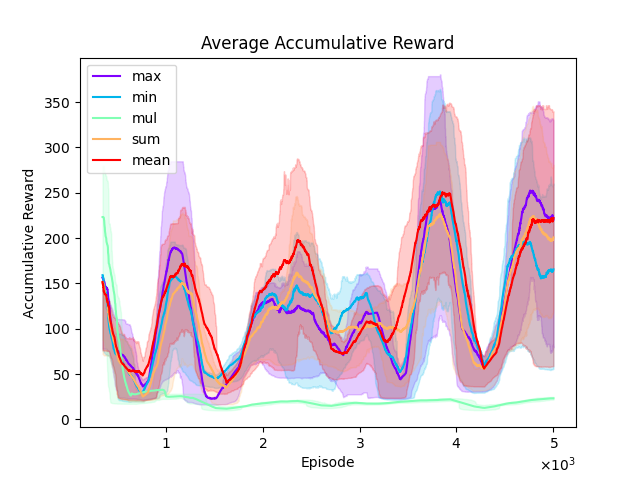
\includegraphics[width=0.75\textwidth]{graphs/aggr/acc_reward_train.png}
	\caption{Training Performance for 36-bus Scenario}
	\label{fig:36-training-performance}
\end{figure}


In the case of the proposed \ac{GRL} techniques, the calibration process failed to improve on performance stability. As observed in the graph in figure \ref{fig:36-training-performance}, this instability is also present during training and shows that the models are failing to generalize the learned information to specific new scenarios. The baseline \ac{SAC} algorithm saw the highest variability of accumulative reward during both training and test phases which is expectable given the absence of a specialized tuning process for this algorithm. We believe the sample efficiency and inherent stability of \ac{SAC}  gave it an additional leverage in this optimization problem.

\begin{table}[h!]
	\centering
	\caption{Test Results for 36-bus Scenario}
	\begin{tabular}{ccccccc}
		\toprule
		\multirow{2}{*}{\textbf{Model}} & \multicolumn{6}{c}{\textbf{Metrics}} \\ 
		\cmidrule(lr){2-7}
		&  \textbf{Avg. CR} & \textbf{Avg. Length} & \textbf{Avg. DOC} & \textbf{Avg. REW} & \textbf{Avg. ST} & \textbf{TT} \\ 
		\midrule
		SAC & 342.84 & 1118.24 & 601896.45 & 5443.65 & 0.0029 & 47.76 \\
		GCN-SAC & 153.77 & 628.19 & 579978.88 & 7356.86 & 0.0097 & 31.11 \\
		GAT-SAC &105.75 & 231.88 & 564739.25 & 7070.78 & 0.0071 & 12.52 \\
		% Add more rows as needed
		\bottomrule
	\end{tabular}
	\label{tab:test-36}
\end{table}

Considering the average step processing time of the model, the \ac{SAC} algorithm also remarkably superior to the proposed models, with a processing time of 29 milliseconds in this scenario, against the average times of 97 and 71 milliseconds of GCN-SAC and GAT-SAC, respectively. The \ac{GRL} techniques were only able to surpass the \ac{SAC} model in training time, but even in this case the results are not positive, since this was mostly due to this algorithm surviving on average a significantly higher amount of steps than the other implementations. This caused the model to train for larger amount of steps than the \ac{GRL} techniques, which also demonstrates the importance of this metric for learning efficiency. By surviving longer into each episode, the \ac{SAC} algorithm was able to face more diverse situations and leverage its features into finding more relevant and generalizable patterns in them. 

\section{Scalability Tests} \label{sec:results-scalability}

To ascertain the scalability of the several implementations, is finally analysed by comparing their performance on the 118-bus scenario. The insights taken from relevant literature, beyond suggesting a promising performance of \ac{GRL}, showed the advantages of these techniques in larger and more complex scenarios. Although the first prospect was not verified in the last subsection, we were still hoping that the feature extraction capabilities of the \ac{GRL} implementations were exacerbated by larger and more complex scenarios. \par

\begin{figure}[ht]
	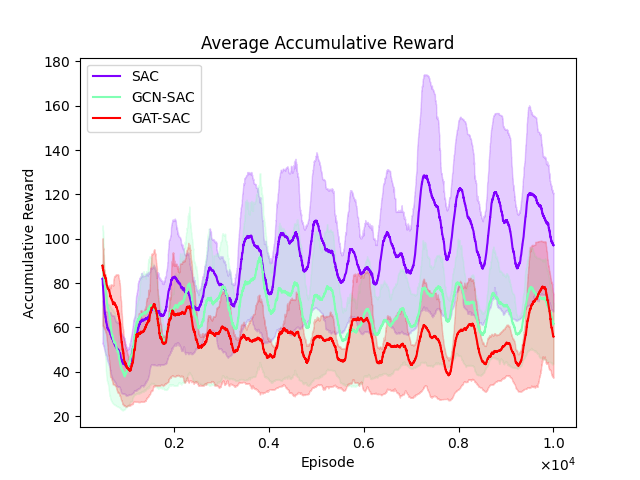
\includegraphics[width=0.75\textwidth]{graphs/118/acc_reward_train.png}
	\caption{Training Performance for the 118-bus Scenario}
	\label{fig:118-training-performance}
\end{figure}

Once more, the proposed implementations did not exceed the \ac{SAC} algortihm in overall performance, as demonstrated by table \ref{tab:test-118}. This model obtained the best average reward per episode and the best convergence, observable in figure \ref{fig:118-training-performance} but at the expense of a slightly shorter survivability than the second-placed GCN-SAC. In this context, the proposed implementations' performance was a lot closer to the baseline, with the GCN-SAC model even showing the best average survival rate in test phase, as shown by the graph in figure \ref{fig:118-sr-val}. However, the results of all models in this metric were generally bad, and this larger scenario aggravated this trend, which it's reflected in the best survival rate of only 19.34 \%. The GAT-SAC model was best in average renewable energy wasted and average daily operating cost. Nevertheless, its low average cumulative reward is mostly explained with its low survival rate. \par

\begin{table}[h!]
	\centering
	\caption{Test Results for the 118-bus Scenario}
	\begin{tabular}{lcccccc}
		\toprule
		\multirow{2}{*}{\textbf{Model}} & \multicolumn{6}{c}{\textbf{Metrics}} \\ 
		\cmidrule(lr){2-7}
		&  \textbf{Avg. CR} & \textbf{Avg. Length} & \textbf{Avg. DOC} & \textbf{Avg. REW} & \textbf{Avg. ST} & \textbf{TT} \\ 
		\midrule
		SAC & 81.98 & 361.92 & 2788763.38 & 4740.03 & 0.0067 & 14.82 \\
		GCN-SAC & 67.85 & 389.82 & 2901439.28 & 5323.58 & 0.0096 & 13.67 \\
		GAT-SAC & 54.31 & 240.28 & 2591733.60 & 4709.37 & 0.0122 & 11.39 \\
		% Add more rows as needed
		\bottomrule
	\end{tabular}
	\label{tab:test-118}
\end{table}

The connection of bad survivability and higher times is also verified in this case although is not as apparent as in the last scenario. The GCN-SAC model had the highest average survival rate during test and also achieved a better training time than the \ac{SAC} algorithm. However, the former model did surpass the \ac{GRL} implementation in average survival rate during training, which explains the higher training time of the \ac{SAC} algorithm. \par

\begin{figure}[ht]
	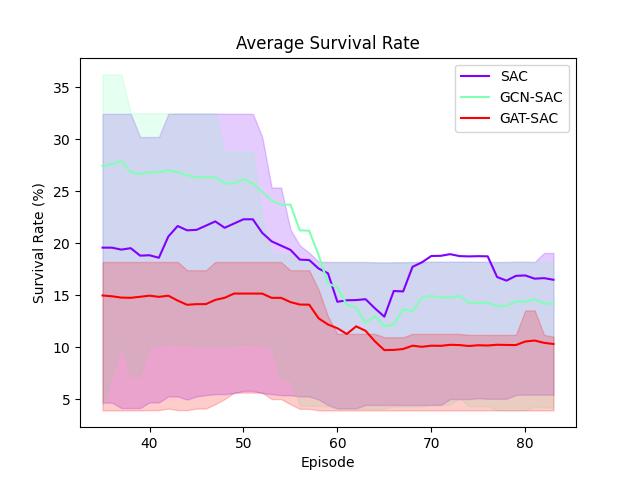
\includegraphics[width=0.75\textwidth]{graphs/118/survival_rate_val.png}
	\caption{Test Survival Rate for the 118-bus Scenario}
	\label{fig:118-sr-val}
\end{figure}

Lastly, our proposed GCN-SAC was able to maintain a similar step processing time in both scenarios, which shows great scalability of this implementation. The \ac{SAC} Model was still superior again, but its step time more than doubled in comparison with the results observed in the 36-bus scenario. GAT-SAC wasn't as consistent as GCN-SAC in this metric, with its processing time considerably increasing.

 
\chapter{Conclusions} \label{chap:conclusions}

In conclusion, this report establishes a solid foundation for implementing and proposing concrete improvements to \ac{GRL} techniques and efficiently solve the problem of \ac{DED} in graph-based environments. \par
We concluded in the literature review, that \ac{GRL} is already a promising solution for \ac{DED}, yielding better performance than other approaches. In general, \acp{GNN} are an ubiquitous method, throughout the gathered literature, for extracting efficient environment topological representations. The identified limitations of existent implementations lie on their lack of: (1) scalability to larger environments, resulting in a significant decrease in computation performance; (2) a seamless integration between \ac{GNN} and \ac{DRL} algorithms and (3) adaptability to real-time topology changes. \par
Moreover, we aim to study how to tackle these limitations by implementing different \ac{GRL} approaches for solving the \ac{DED} problem and conducting a comparative study between the different techniques. The implementations will be compromised of various combinations of \acp{GNN}, for efficiently extracting the relevant environment features, and \ac{DRL} algorithms for mapping the extracted representations into optimal action sequences. Case studies will be carried out within different size modified IEEE bus systems for testing the various models and confront their results. Lastly, the models will be analysed considering their training efficiency, computational performance, dispatch efficiency, scalability to large scenarios and adaptability to topological changes. Based on the conclusions drawn from the comparative study, we will propose a \ac{GRL} that implements concrete enhancements.

\section{Main Contributions}

In this section, we list the expected contributions derived from this work on a Scientific, Technological and Application levels:
\begin{description}
	\item[Scientific] A systematic and comparative study of different \ac{GRL} approaches. This fills the research gap for systematic studies comparing different proposed techniques. Furthermore, this work will bring a clearer insight regarding the best practices on implementing \ac{GRL} models
	\item[Technological] A model resulting from this study with concrete improvements over the current \ac{GRL} techniques proposed so far and tackling their limitations. Beyond this, 
	\item[Application] An efficient solution for the \ac{DED} problem with \ac{GRL} algorithms, compromising significant contribution to the research on \ac{DED} systems in complex scenarios
\end{description}

\section{Future Work}

While this work extensively explored potential improvements in \ac{GRL} techniques and their applications to the \ac{DED} problem, the scope of the issue is vast, and several areas for improvement were left unaddressed due to time and planning constraints. The main future concerns are aligned with improving the performance of the model and further investigating other potential enhancements to the \ac{GRL} techniques. \par

Firstly, it would be valuable to explore additional \ac{DRL} and \ac{GNN} implementations to compare with the results obtained from the studied models. For example, alternative combinations of \ac{GNN} models like GraphSAGE and \ac{DRL} algorithms such as PPO and DDPG might yield better performance than those tested in this study. Additionally, the author is keen to compare the studied single-agent \ac{GRL} technique with multi-agent systems in the \ac{DED} problem. Given their distinct perspectives on the issue, such a comparison could provide valuable insights into the effectiveness of each approach. \par

Given the complexity and diversity of modern power systems, it would also be worthwhile to consider additional elements, such as \acf{ESS} storage, which were excluded to avoid overly complicating the environmental dynamics. Moreover, investigating how voltage control could enhance the agent's reliability and, consequently, the survivability of models appears to be a relevant area for further study. \par

Finally and most importantly, further experimentation and calibration, especially with larger scenarios, might be necessary to understand the failures of this work's approach on \ac{GRL} techniques. There is still promising evidence from the literature of their performance on graph-based scenarios, but the study and analysis that was conducted failed to reach that conclusion. 



%%----------------------------------------
%% Final materials
%%----------------------------------------

%% Bibliography
%% Comment the next command if BibTeX file not used
%% bibliography is in ``myrefs.bib''
\PrintBib{bibliography}

%% 2021-07-20: change
%% comment next 2 commands if numbered appendices are not used
\appendix
\chapter{Appendix} \label{appendix}

\section{Limit Infeasible Curtail Action Experiment Results}

\begin{figure}[H]
	\centering
	\subfloat{}{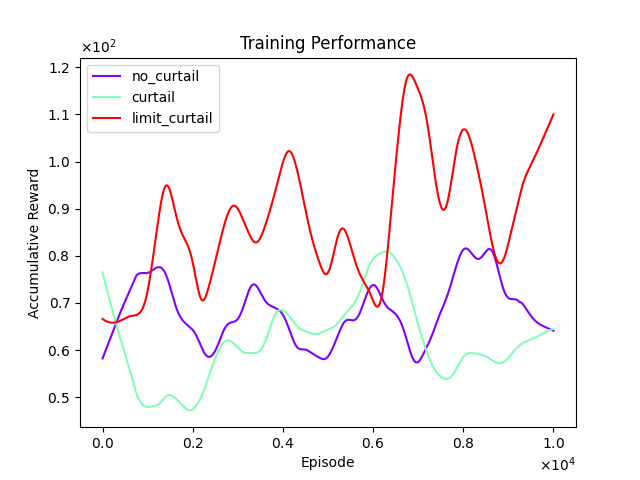
\includegraphics[width=.45\textwidth]{graphs/curtail_limit/training_performance.png}}
	\hskip1ex
	\subfloat{}{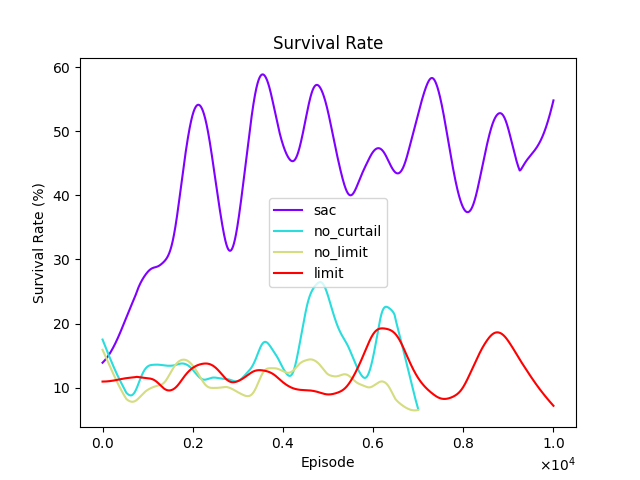
\includegraphics[width=.45\textwidth]{graphs/curtail_limit/survival_rate.png}} 
	\vfill
	\subfloat{}{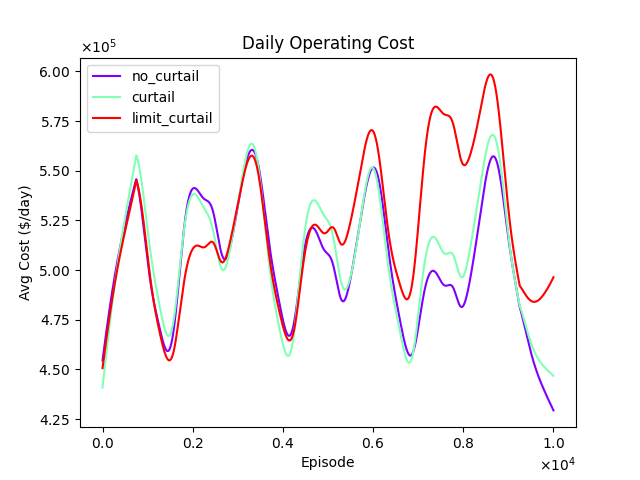
\includegraphics[width=.45\textwidth]{graphs/curtail_limit/daily_cost.png}} \hskip1ex
	\subfloat{}{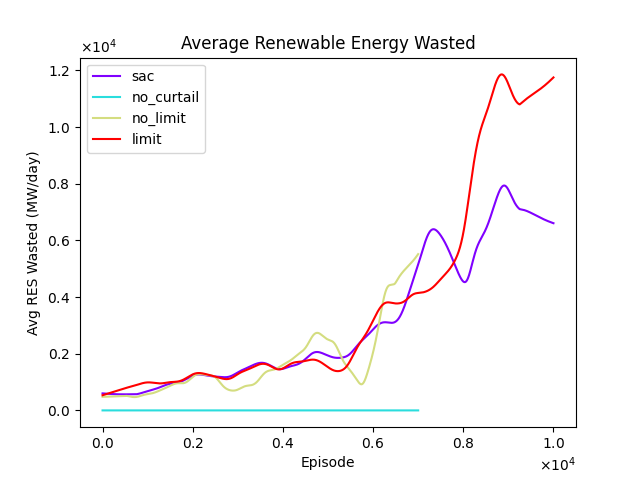
\includegraphics[width=.45\textwidth]{graphs/curtail_limit/res_wasted.png}} 
	\caption{Training Results of the Experiments concerning Limit Infeasible Curtail Actions.}
	\label{fig:curtail-train}
\end{figure}

\begin{table}[ht]
	\centering
	\begin{tabularx}{\textwidth}{|l|X|X|X|X|X|}
		\hline
		\textbf{Model} & \textbf{Avg. Accumulative Reward}& \textbf{Avg. Length (Steps)} & \textbf{Avg Daily Operating Cost (€)} & \textbf{Avg. Renewables Wasted (MW/day)} & \textbf{Total Time (Seconds)}\\
		\hline
		no\_curtail & 68.87 & 225.46 & 533238.32 & 0.0 & 812.81\\
		curtail & 60.81 & 108.27 & 551028.29 & 4565.01 & 510.97 \\
		limit\_curtail & 78.62 & 759.82 & 575798.57 & 7640.76 & 2329.76 \\
		\hline
	\end{tabularx}
	\caption{Validation Results of the Experiments concerning Limit Infeasible Curtail Actions.}
	\label{fig:curtail-val}
\end{table}

\section{Curtailment Lower Limit Smoothing}

\begin{figure}[H]
	\centering
	\subfloat{}{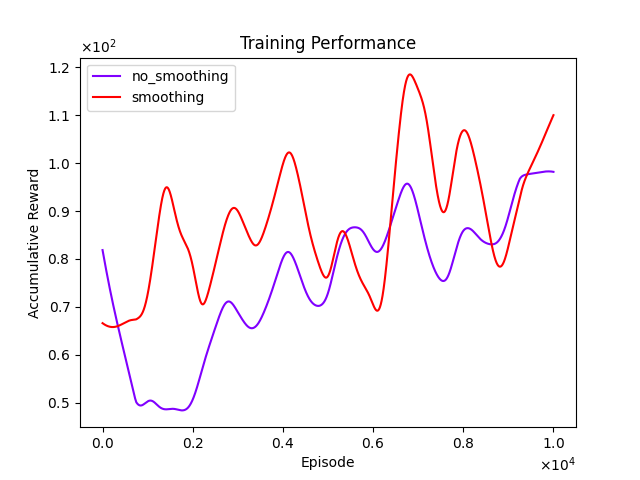
\includegraphics[width=.45\textwidth]{graphs/curtail_smooth/training_performance.png}}
	\hskip1ex
	\subfloat{}{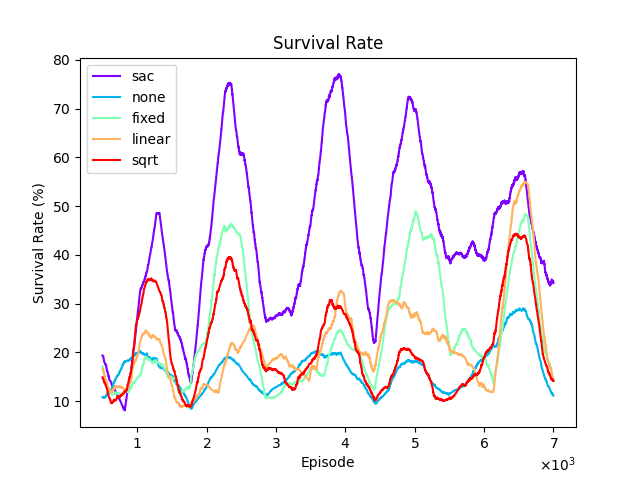
\includegraphics[width=.45\textwidth]{graphs/curtail_smooth/survival_rate.png}} 
	\vfill
	\subfloat{}{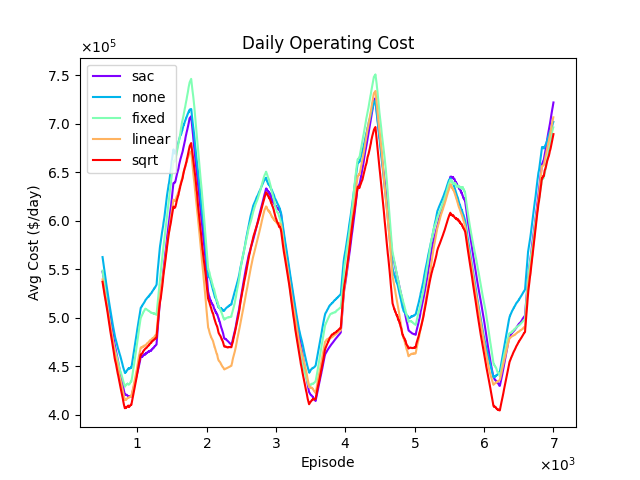
\includegraphics[width=.45\textwidth]{graphs/curtail_smooth/daily_cost.png}} \hskip1ex
	\subfloat{}{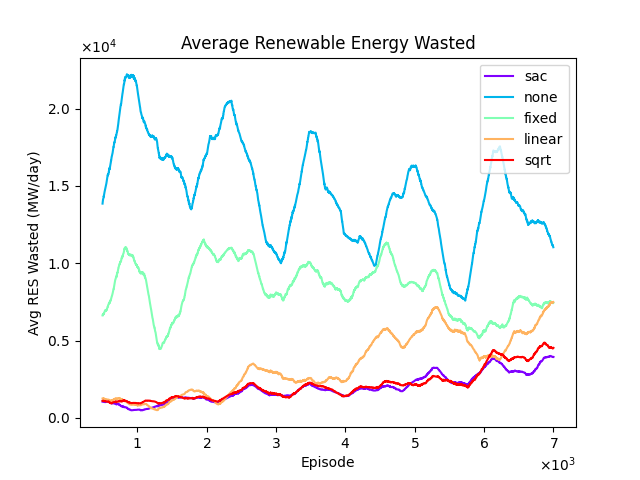
\includegraphics[width=.45\textwidth]{graphs/curtail_smooth/res_wasted.png}} 
	\caption{Training Results of the Experiments concerning Curtailment Lower Limit Smoothing.}
	\label{fig:curtail-smooth-train}
\end{figure}

\begin{table}[ht]
	\centering
	\begin{tabularx}{\textwidth}{|l|X|X|X|X|X|}
		\hline
		\textbf{Model} & \textbf{Avg. Accumulative Reward}& \textbf{Avg. Length (Steps)} & \textbf{Avg Daily Operating Cost (€)} & \textbf{Avg. Renewables Wasted (MW/day)} & \textbf{Total Time (Seconds)}\\
		\hline
		no\_smoothing & 94.91 & 476.48 & 565094.39 & 10106.84 & 3011.93 \\
		smoothing & 78.62 & 759.82 & 575798.57 & 7640.76 & 2329.76 \\
		\hline
	\end{tabularx}
	\caption{Validation Results of the Experiments concerning Limit Infeasible Curtail Actions.}
	\label{fig:curtail-val}
\end{table}

\section{Reward Experiments}

\begin{figure}[H]
	\centering
	\subfloat{}{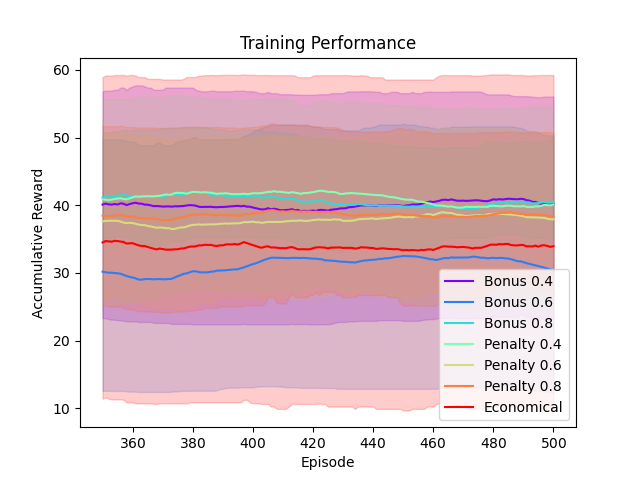
\includegraphics[width=.45\textwidth]{graphs/reward/training_performance.png}}
	\hskip1ex
	\subfloat{}{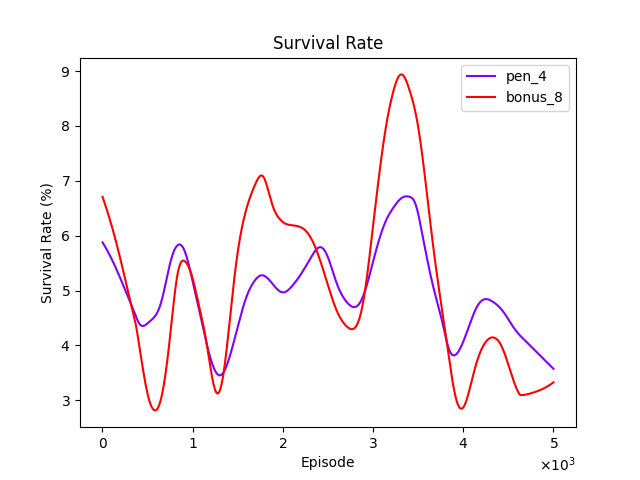
\includegraphics[width=.45\textwidth]{graphs/reward/survival_rate.png}} 
	\vfill
	\subfloat{}{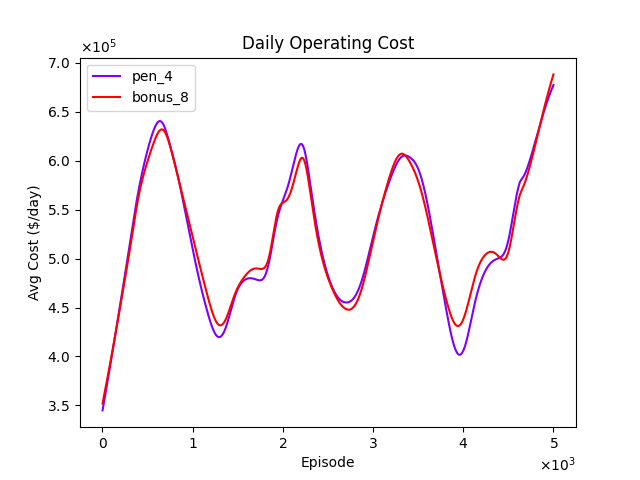
\includegraphics[width=.45\textwidth]{graphs/reward/daily_cost.png}} \hskip1ex
	\subfloat{}{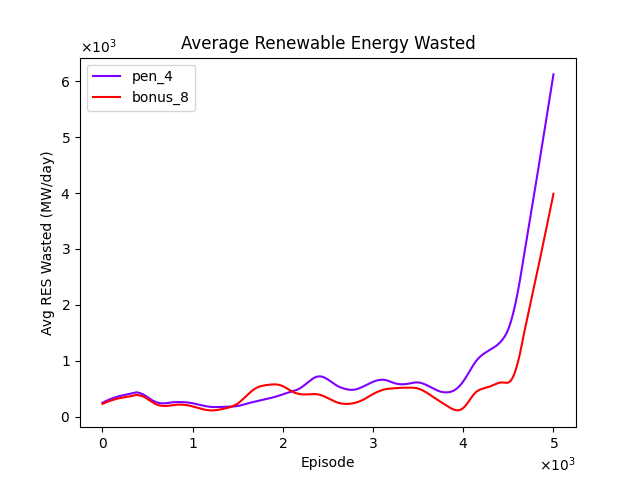
\includegraphics[width=.45\textwidth]{graphs/reward/res_wasted.png}} 
	\caption{Training Results of the best Penalty and Bonus Factor Rewards.}
	\label{fig:reward-best-train}
\end{figure}
\begin{figure}[H]
	\centering
	\subfloat{}{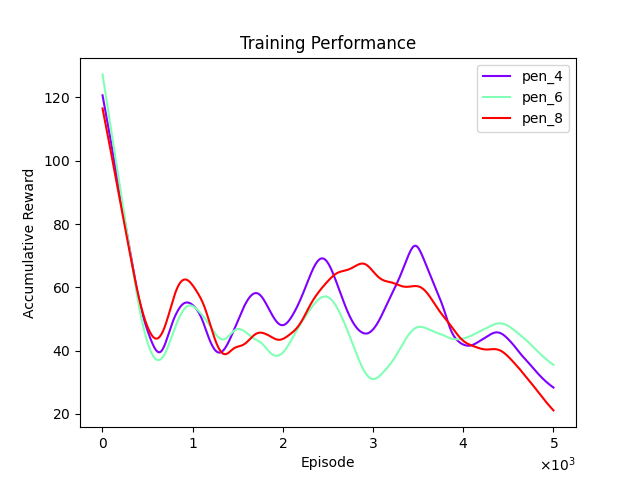
\includegraphics[width=.45\textwidth]{graphs/reward/penalty/training_performance.png}}
	\hskip1ex
	\subfloat{}{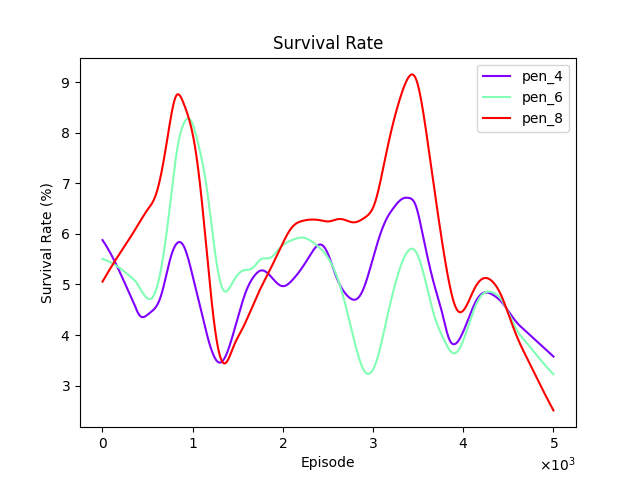
\includegraphics[width=.45\textwidth]{graphs/reward/penalty/survival_rate.png}} 
	\vfill
	\subfloat{}{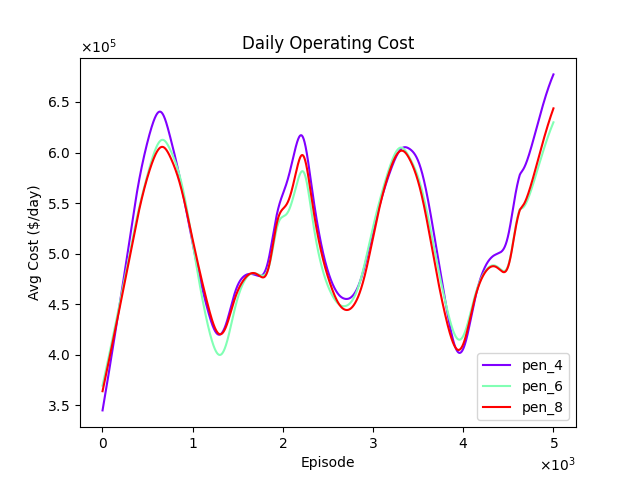
\includegraphics[width=.45\textwidth]{graphs/reward/penalty/daily_cost.png}} \hskip1ex
	\subfloat{}{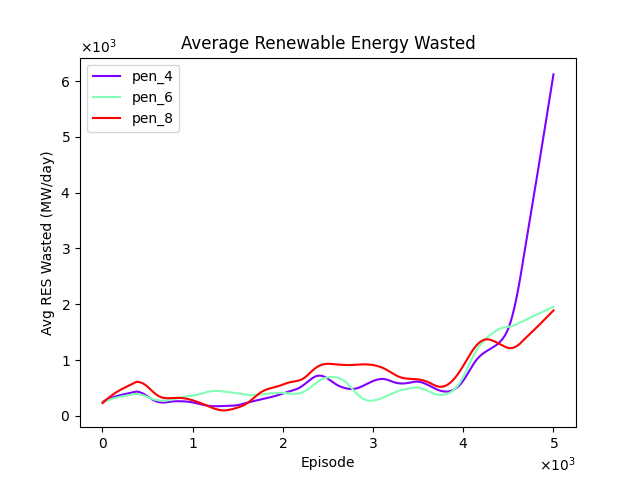
\includegraphics[width=.45\textwidth]{graphs/reward/penalty/res_wasted.png}} 
	\caption{Training Results of the Penalty Factor Rewards.}
	\label{fig:reward-pen-train}
\end{figure}

\begin{figure}[H]
	\centering
	\subfloat{}{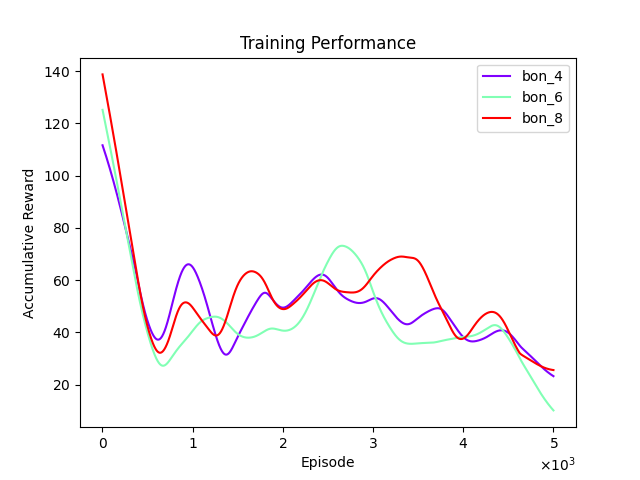
\includegraphics[width=.45\textwidth]{graphs/reward/bonus/training_performance.png}}
	\hskip1ex
	\subfloat{}{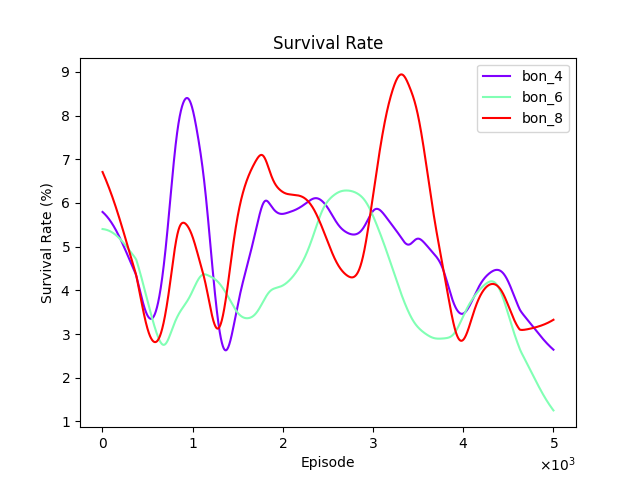
\includegraphics[width=.45\textwidth]{graphs/reward/bonus/survival_rate.png}} 
	\vfill
	\subfloat{}{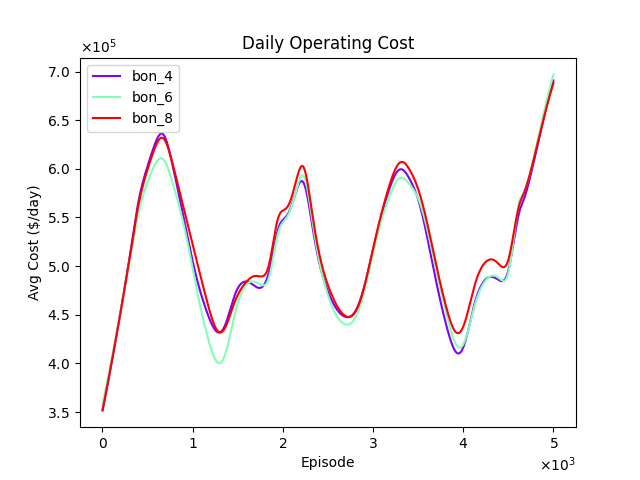
\includegraphics[width=.45\textwidth]{graphs/reward/bonus/daily_cost.png}} \hskip1ex
	\subfloat{}{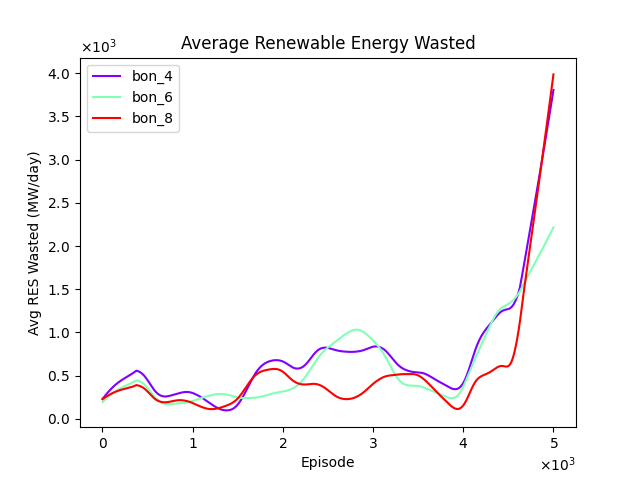
\includegraphics[width=.45\textwidth]{graphs/reward/bonus/res_wasted.png}} 
	\caption{Training Results of the Bonus Factor Rewards.}
	\label{fig:reward-bon-train}
\end{figure}

\begin{table}[ht]
	\centering
	\begin{tabularx}{\textwidth}{|l|X|X|X|X|X|}
		\hline
		\textbf{Model} & \textbf{Avg. Accumulative Reward}& \textbf{Avg. Length (Steps)} & \textbf{Avg Daily Operating Cost (€)} & \textbf{Avg. Renewables Wasted (MW/day)} & \textbf{Total Time (Seconds)}\\
		\hline
		pen\_4 & 40.57 & 80.75 & 565893.63 & 4100.20 & 230.99 \\
		pen\_6 & 37.54 & 81.40 & 558362.82 & 2570.71 & 231.09 \\
		pen\_8 & 38.22 & 76.35 & 555582.14 & 2612.34 & 222.58 \\
		bon\_4 & 40.13 & 76.23 & 565757.16 & 3723.72 & 223.90 \\
		bon\_6 & 30.78 & 55.06 & 566786.07 & 2750.34 & 189.01 \\
		bon\_8 & 40.88 & 96.43 & 560927.60 & 3115.18 & 256.59 \\
		\hline
	\end{tabularx}
	\caption{Validation Results of the Experiments concerning Limit Infeasible Curtail Actions.}
	\label{fig:curtail-val}
\end{table}

\section{Experiments on the \ac{GNN} Parameters \textit{act\_first} and \textit{improved}}

\begin{figure}[H]
	\centering
	\subfloat{}{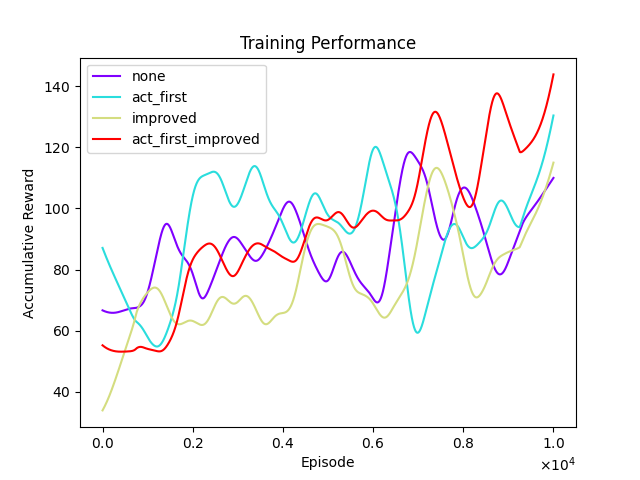
\includegraphics[width=.45\textwidth]{graphs/act_first_improved/training_performance.png}}
	\hskip1ex
	\subfloat{}{\includegraphics[width=.45\textwidth]{graphs/act_first_improved/survival_rate.png}} 
	\vfill
	\subfloat{}{\includegraphics[width=.45\textwidth]{graphs/act_first_improved/daily_cost.png}} \hskip1ex
	\subfloat{}{\includegraphics[width=.45\textwidth]{graphs/act_first_improved/res_wasted.png}} 
	\caption{Training Results of the act\_first and improved Parameter Tests.}
	\label{fig:act-first-improved-train}
\end{figure}

\begin{comment}
\begin{table}[ht]
	\centering
	\begin{tabularx}{\textwidth}{|l|X|X|X|X|X|}
		\hline
		\textbf{Model} & \textbf{Avg. Accumulative Reward}& \textbf{Avg. Length (Steps)} & \textbf{Avg Daily Operating Cost (€)} & \textbf{Avg. Renewables Wasted (MW/day)} & \textbf{Total Time (Seconds)}\\
		\hline
		none & & & & & \\
		act\_first & & & & & \\
		improved & & & & & \\
		act\_first\_improved & & & & &  \\
		\hline
	\end{tabularx}
	\caption{Validation Results of the Experiments concerning Limit Infeasible Curtail Actions.}
	\label{fig:curtail-val}
\end{table}
\end{comment}

\section{Experiments on the number of \ac{GNN} layers}

\begin{figure}[H]
	\centering
	\subfloat{}{\includegraphics[width=.45\textwidth]{graphs/layers/training_performance.png}}
	\hskip1ex
	\subfloat{}{\includegraphics[width=.45\textwidth]{graphs/layers/survival_rate.png}} 
	\vfill
	\subfloat{}{\includegraphics[width=.45\textwidth]{graphs/layers/daily_cost.png}} \hskip1ex
	\subfloat{}{\includegraphics[width=.45\textwidth]{graphs/layers/res_wasted.png}} 
	\caption{Training Results of models with 2, 3, 4 and 5 \ac{GNN} Layers}
	\label{fig:gnn-layers-train}
\end{figure}

\begin{comment}
\begin{table}[ht]
	\centering
	\begin{tabularx}{\textwidth}{|l|X|X|X|X|X|}
		\hline
		\textbf{Model} & \textbf{Avg. Accumulative Reward}& \textbf{Avg. Length (Steps)} & \textbf{Avg Daily Operating Cost (€)} & \textbf{Avg. Renewables Wasted (MW/day)} & \textbf{Total Time (Seconds)}\\
		\hline
		2 & & & & & \\
		3 & & & & & \\
		4 & & & & & \\
		5 & & & & & \\
		\hline
	\end{tabularx}
	\caption{Validation Results of the Experiments concerning Limit Infeasible Curtail Actions.}
	\label{fig:curtail-val}
\end{table}
\end{comment}


\section{Experiments on the number of \ac{GAT} Heads}

\begin{figure}[H]
	\centering
	\subfloat{}{\includegraphics[width=.45\textwidth]{graphs/layers/training_performance.png}}
	\hskip1ex
	\subfloat{}{\includegraphics[width=.45\textwidth]{graphs/layers/survival_rate.png}} 
	\vfill
	\subfloat{}{\includegraphics[width=.45\textwidth]{graphs/layers/daily_cost.png}} \hskip1ex
	\subfloat{}{\includegraphics[width=.45\textwidth]{graphs/layers/res_wasted.png}} 
	\caption{Training Results of models with 1, 2 and 3 \ac{GAT} Heads}
	\label{fig:gat-heads-train}
\end{figure}

\begin{comment}
\begin{table}[ht]
	\centering
	\begin{tabularx}{\textwidth}{|l|X|X|X|X|X|}
		\hline
		\textbf{Model} & \textbf{Avg. Accumulative Reward}& \textbf{Avg. Length (Steps)} & \textbf{Avg Daily Operating Cost (€)} & \textbf{Avg. Renewables Wasted (MW/day)} & \textbf{Total Time (Seconds)}\\
		\hline
		1 & & & & & \\
		2 & & & & & \\
		3 & & & & & \\
		\hline
	\end{tabularx}
	\caption{Validation Results of the Experiments concerning Limit Infeasible Curtail Actions.}
	\label{fig:curtail-val}
\end{table}
\end{comment}

%% Index
%% Uncomment next command if index is required
%% don't forget to run ``makeindex thesis'' command
%\PrintIndex

\end{document}
